\documentclass{article}
\usepackage[utf8]{inputenc}
\usepackage{setspace}
\usepackage{graphicx}
\usepackage{titling}
\usepackage{textcomp}
\usepackage[nottoc]{tocbibind}
\usepackage{tocloft}
\usepackage{natbib}
\usepackage{amsmath}
\usepackage{amssymb}
\usepackage{subcaption}
\usepackage{multicol}
\usepackage{tabulary}
%\usepackage{fontspec}
\renewcommand{\cftsecleader}{\cftdotfill{\cftdotsep}}

\usepackage[margin=1.5in]{geometry}
\addtolength{\topmargin}{-0.5in}
\addtolength{\textheight}{1.0in}

\doublespacing
\newenvironment{bottompar}{\par\vspace*{\fill}}{}

\renewcommand{\contentsname}{\center{Table of Contents}}

\title{Real-time Video Alignment and Fusion Using Feature Detection on FPGA Devices}

\author{Robert Haywood Taglang}

\begin{document}
\pagenumbering{gobble}
\begin{titlingpage}
    \vspace*{\fill}
    \begin{center}
        \textbf{\thetitle}
        
        \hfill \\
        \hfill \\
        
        A Thesis \\
        Submitted to the Faculty \\
        of \\
        Drexel University \\
        by \\
        \theauthor \\
        in partial fulfillment of the \\
        requirements for the degree \\
        of \\
        Master of Science in Computer Engineering \\
        June 2017 \\
    \end{center}
    
    \vspace*{\fill}
    
    \begin{figure*}[!b]
    	\centering
       	
\includegraphics[width=0.35\textwidth]{drexel-vert-blue}
    \end{figure*}
\end{titlingpage}

\begin{center}
	\vspace*{\fill}
	
	\textcopyright\  Copyright 2017
	
	Robert H. Taglang. All Rights Reserved.
	
	\vspace*{\fill}
\end{center}
\clearpage

\pagenumbering{roman}
\setcounter{page}{2}
\begin{center}
    \tableofcontents
    \clearpage
    
    \listoftables
    \clearpage
    
    \listoffigures
\end{center}
\clearpage

\hfill \\
\hfill \\
\hfill \\
\hfill \\

\addcontentsline{toc}{section}{Abstract}

\begin{abstract}
    \singlespacing
    \centering
    \thetitle \\
    \theauthor \\
    Prawat Nagvajara, Ph.D. \\
    
    \hfill \\
    \hfill \\
    \hfill \\
    
    \doublespacing
    Video fusion functions as a way to combine the important or useful parts of two or more sequences of images. The scenario presented is the use of Laplacian fusion to produce a single video composed of the fields of view of two cameras whose areas of focus differ substantially. This is not a useful real-time strategy unless the fields can be aligned. This thesis presents a system for detecting features using an FPGA implementation of SURF (Speeded-Up Robust Features), and aligning video streams by applying a transform generated from the key features. 
\end{abstract}

\clearpage

\pagenumbering{arabic}

\section{Background}

\subsection{Introduction}

The fusion of data from two or more sensors has been well-researched \cite{wang_multi-focus_2011} \cite{li_multi-sensor_1994}, though these approaches typically discuss the process of fusing images which have been pre-aligned. Pre-computed transforms used to align the frames of two cameras are not robust to variations. Some approaches have made use of additional hardware sensors in order to correct against these variations \cite{chappell_exploiting_2006}. The approach presented in this thesis seeks to perform this correction in real time, completely in hardware, using feature detection on a Field Programmable Gate Array (FPGA) using the design shown in Figure \ref{fig_block_diagram}.

\begin{figure}[h]
	\centering
	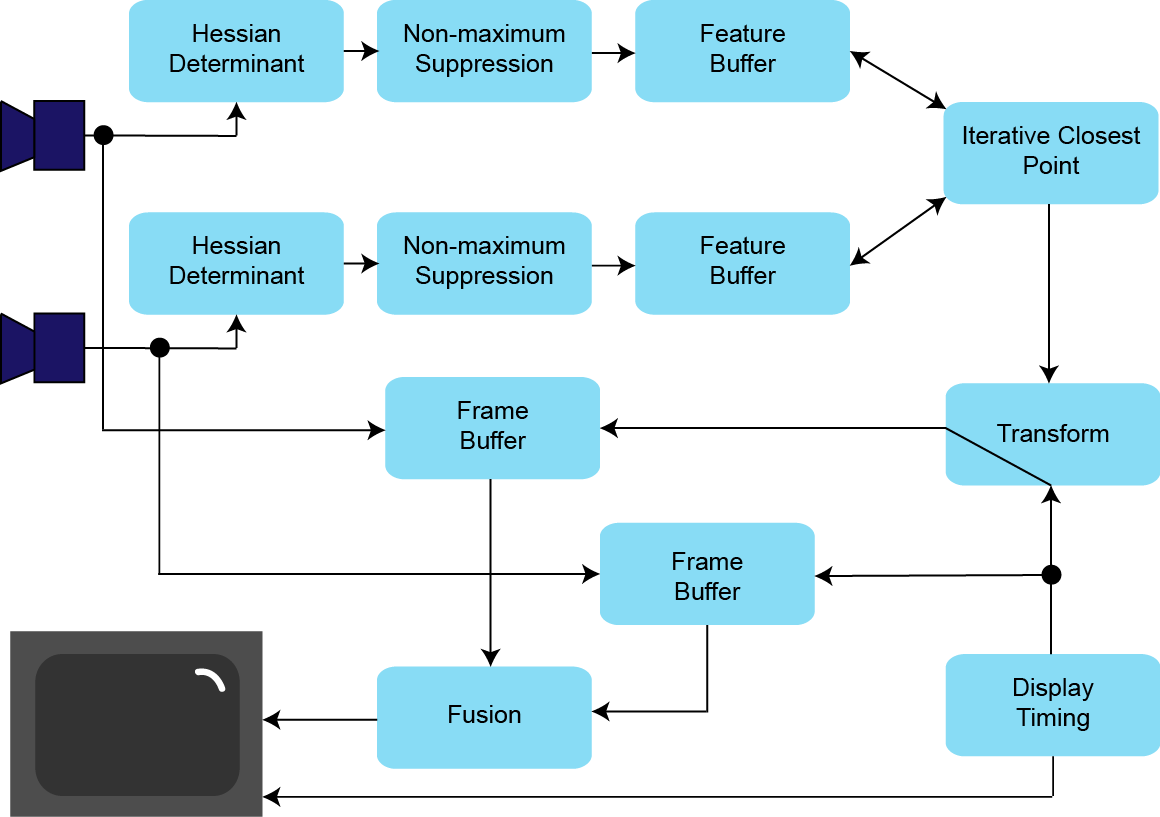
\includegraphics[width=0.8\textwidth]{figures/block/blockdiagram}
	\caption{Block diagram of the proposed system for alignment and fusion}
	\label{fig_block_diagram}
\end{figure}

In order to align two images, one is treated as the reference image, and the other is the transform image which needs to be transformed to be aligned with the reference image. As such the problem can be broken into four major components. 

\begin{enumerate}
	\item Detecting feature points in the two images
	\item Computing the transform which maps the transform image into the space of the reference image
	\item Applying the computed transform to the transform image
	\item Fusion of the reference and transformed image
\end{enumerate}

Feature points are detected using some of the techniques from Speeded-up Robust Features (SURF) which makes use of Hessian determinants to detect points of interest in multiple scale spaces. High magnitude features are stored in a buffer to be used for computing the transform.

Once the feature points for the two images have been computed and stored in the buffer, the points from the transform image are mapped to their closest point in terms of euclidean distance from the reference set. An orthogonal projection from the transform points to the reference points is created with the transform as the unknown. Singular value decomposition is used to compute the pseudo-inverse of the matrix containing the reference points so it can be premultiplied by the matrix containing the transform points. The result of this product is the transform matrix which maps transform points to reference points with the error minimized in a least-squares sense. This process may need to be repeated multiple times to converge to a local error minimum, a process referred to as iterative closest point.

As the image data streams into hardware, the data is buffered into memory. With the transform computed, the desired address for the output image is decomposed into $x$ and $y$ coordinates, which are transformed and then reformed back into an address which is used to select pixels from the data in memory. In this way, the transform is applied to align the transform image with the reference image.

Finally, the technique of Laplacian fusion is used to combine the aligned images. It effectively selects the highest frequency components from the two images in order to create an output image where the sharpest, focused parts of the two images are combined into one image.

This process is applied continuously in real time. As the data from the camera data streams in, it produces a single fused output image for display with minimal latency. The design choice to use a FPGA rather than a GPU or some other software based approach was made due to the advantages gained from operating with custom embedded hardware over more rigid architectures. Overall, custom hardware implementations will always beat off-the-shelf components in terms of size, weight, and power consumption.

\subsection{Laplacian Fusion}

Laplacian pyramids of images have their origin as a strategy for image encoding \cite{burt_laplacian_1983}. A gaussian blur is applied to the image, and the image is downsampled to half of its original size. In this context, Gaussian blur refers to applying kernel convolution to this image with a Gaussian kernel. Likewise, a box blur is the application of a uniformly valued, normalized kernel through kernel convolution. Downsampling refers the process of halving the resolution of the image by combining adjacent pixels. Upsampling is the process of doubling the resolution of the image and interpolating the missing values in the new image. The process of blurring and downsampling can be repeated on the resulting image to create a sequence of images representing the original in different scale spaces. This sequence of blurred and downsampled images is known as a Gaussian pyramid. An illustration of a Guassian pyramid for an example image can be seen in Figure \ref{fig_pepper_gaussian_pyramid}.

\begin{figure}[h]
	\centering
	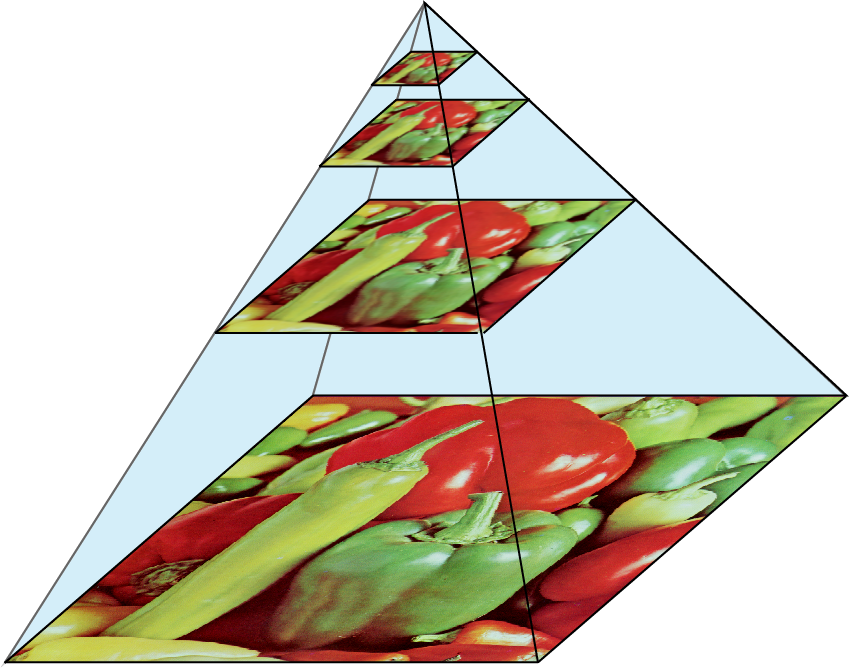
\includegraphics[width=0.6\textwidth]{figures/peppers/gaussian_pyramid}
	\caption{Gaussian pyramid of an example image}
	\label{fig_pepper_gaussian_pyramid}
\end{figure}

The Laplacian pyramid is one which can be used for reconstruction of the original image. At each level above the lowest level of the Gaussian pyramid, the level below is upsampled to match the scale of the current level. The difference between the upsampled image and the current scale level image is known as the Laplacian of the image. The sum of the upsampled lower level and the Laplacian is the original image. At a single level, the Laplacian can be thought of as the error introduced by applying a Gaussian and Box filter. A diagram illustrating a Laplacian pyramid can be seen in Figure \ref{fig_pepper_laplacian_pyramid}. In Figure \ref{fig_pepper_laplacian_pyramid}, the $G\downarrow$ operator refers to applying the Gaussian blur and downsampling, the $\uparrow$ operator refers to upsampling the input image, and the $-$ operator refers to computing the difference of the two input 
images on each channel.
\begin{figure}[h]
	\centering
	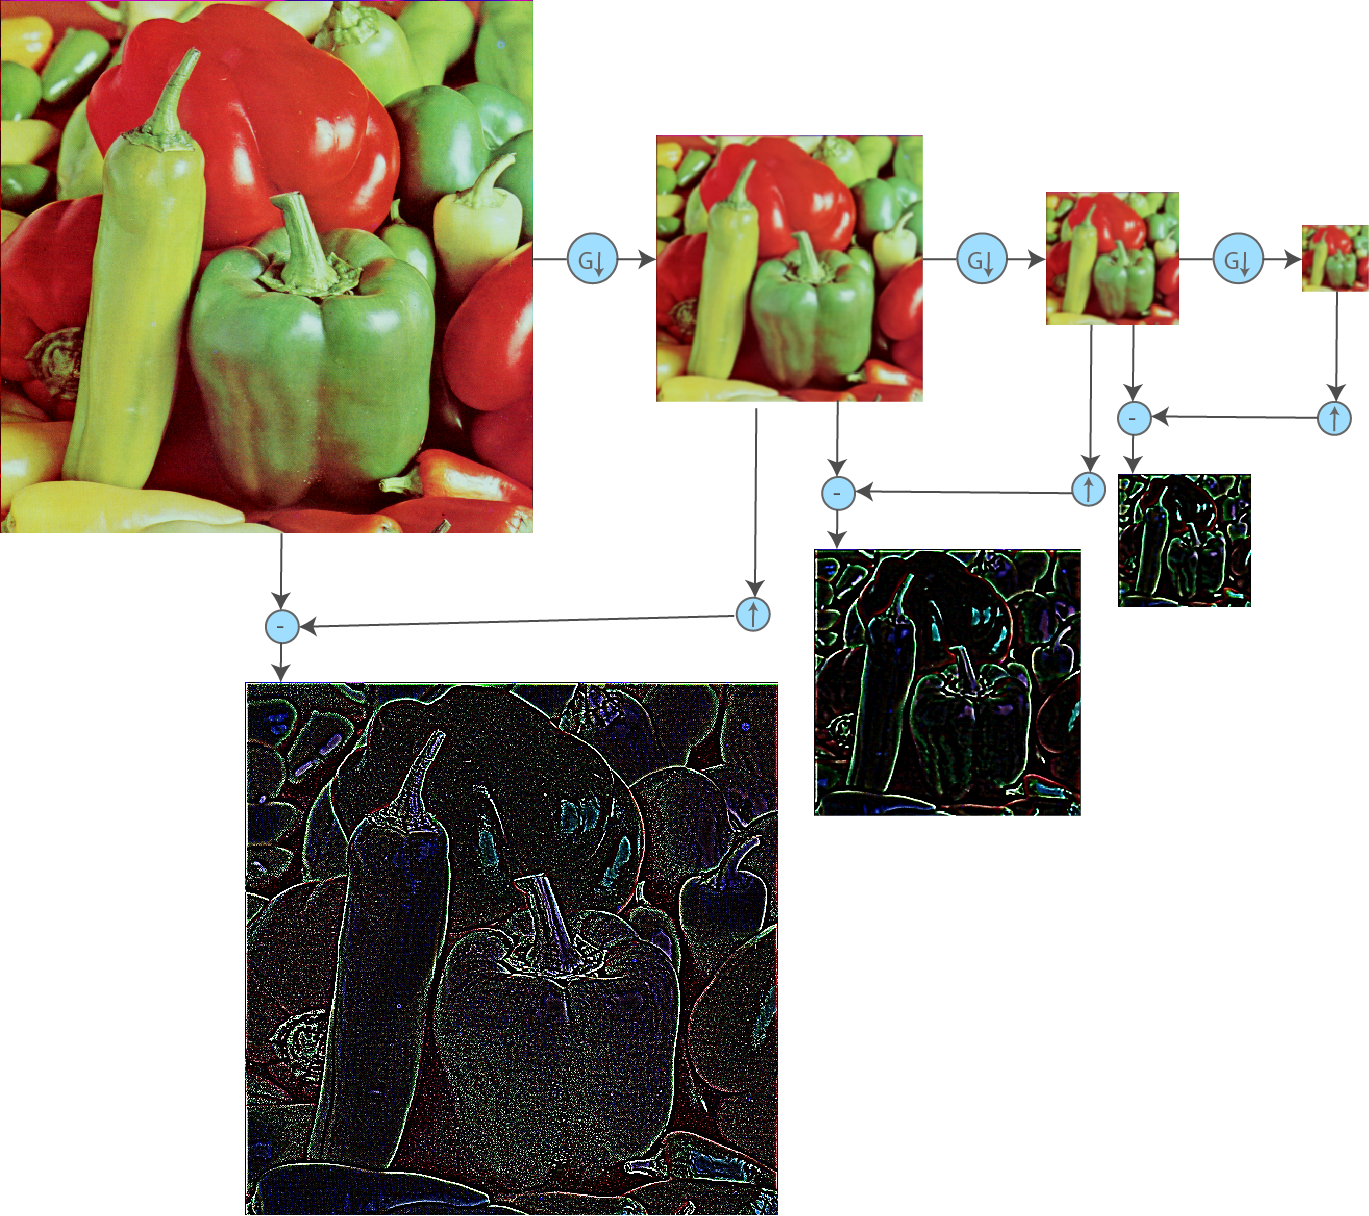
\includegraphics[width=\textwidth]{figures/peppers/laplacian_pyramid}
	\caption{Laplacian pyramid of an example image}
	\label{fig_pepper_laplacian_pyramid}
\end{figure}

The property of the Laplacian that makes it ideal for fusion is its ability to capture the high frequency components in an image through the use of very simple kernel operators that are easily implemented in hardware. The difference between a blurred image and the original will have higher magnitude in the areas where the image was sharpest.

The fusion of two images can be thought of as a function of the two images $X$ and $Y$ of dimension $M \times N$ where $Z = f(X, Y)$, a single image of dimension $M \times N$. A naive approach to fusion would be to compute the Laplacians and use their magnitudes to select a pixel from either $X$ or $Y$ as shown in Equation \ref{eq_naive_fusion}. In this context, $|L(x)|$ represents the absolute value of the Laplacian of the input.

\begin{equation}
Z(i,j)=
\begin{cases}
X(i,j) & |L(X(i,j))| \ge |L(Y(i,j))| \\
Y(i,j) & otherwise
\end{cases}
\label{eq_naive_fusion}
\end{equation}

This approach does not account for variations in colorspace between the two images. Consider the images in Figure \ref{fig_peppers_lr}. The more saturated image will likely have a higher valued Laplacian in some parts simply because it is brighter, therefore having higher magnitudes at individual pixels. This approach also will not facilitate smooth stitching of the images. Contiguous regions of selection from one image will be adjacent to regions from the other with no transition, producing a grainy effect at areas of high frequency. The result of this naive fusion can be seen in Figure \ref{fig_naive_fusion} which exhibits the flaws of this approach.

\begin{figure}[h]
	\centering
	\begin{subfigure}[b]{0.45\textwidth}
		\centering
		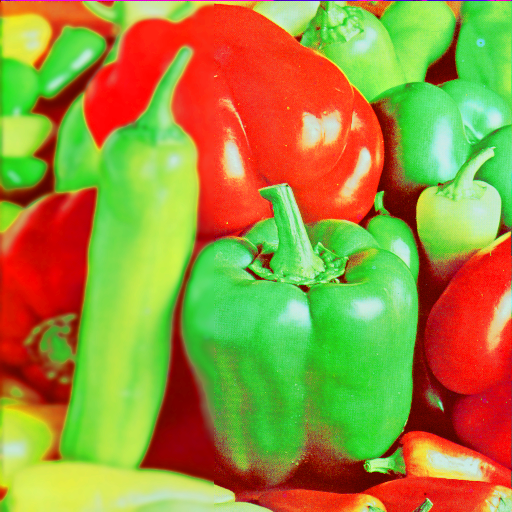
\includegraphics[width=\textwidth]{figures/peppers/peppers_blur_left}
		\caption{Blurred on the left; more saturated}
	\end{subfigure}
	\begin{subfigure}[b]{0.45\textwidth}
		\centering
		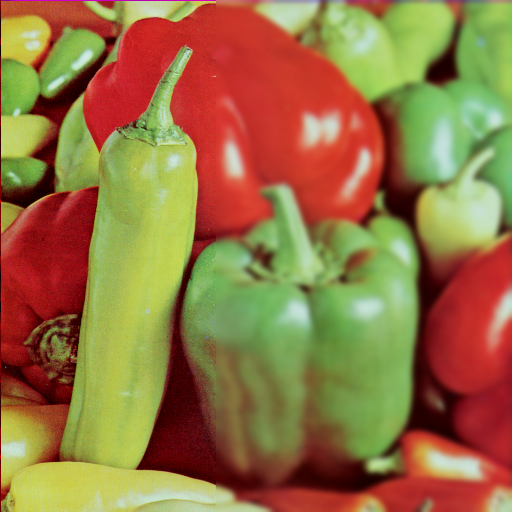
\includegraphics[width=\textwidth]{figures/peppers/peppers_blur_right}
		\caption{Blurred on the right; more neutral}
	\end{subfigure}
	\caption{Two images of the same scene with variations in sharpness and colorspace}
	\label{fig_peppers_lr}
\end{figure}

\begin{figure}[h]
	\centering
	\begin{subfigure}[b]{0.45\textwidth}
		\centering
		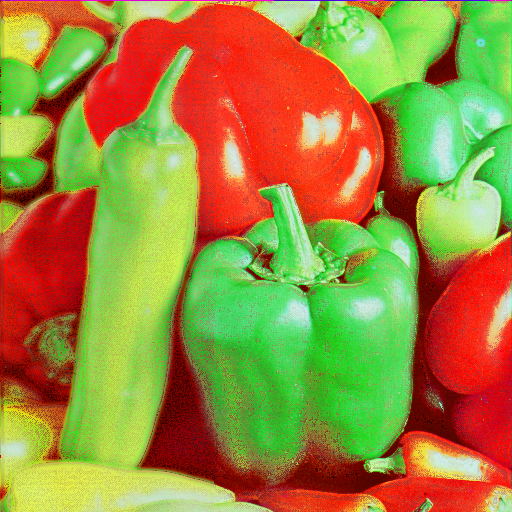
\includegraphics[width=\textwidth]{figures/peppers/peppers_fused_naive}
		\caption{Fusion using the naive approach}
		\label{fig_naive_fusion}
	\end{subfigure}
	\begin{subfigure}[b]{0.45\textwidth}
		\centering
		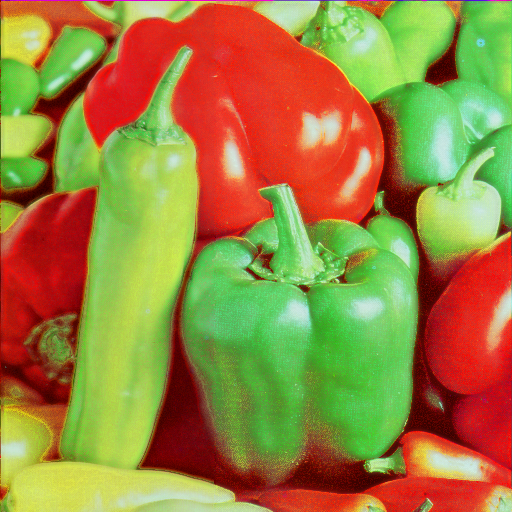
\includegraphics[width=\textwidth]{figures/peppers/peppers_fused}
		\caption{Fusion using weighted sum}
		\label{fig_weighted_fusion}
	\end{subfigure}
	\caption{Fusion of the images in Figure \ref{fig_peppers_lr} using a naive selection and weighted sum approach}
\end{figure}

A more correct approach would involve using the Laplacian in a weighted sum to combine the pixels of the images, rather than simply selecting them, as shown in Equation \ref{eq_weighted_fusion}.

\begin{equation}
Z(i,j) = \frac{|L(X(i,j))|}{|L(X(i,j))| + |L(Y(i,j))|} \cdot X(i,j) + \frac{|L(Y(i,j))|}{|L(X(i,j))| + |L(Y(i,j))|} \cdot Y(i,j)
\label{eq_weighted_fusion}
\end{equation}

The result of this weighted sum approach can be seen in Figure \ref{fig_weighted_fusion} which exhibits a reduction in graininess from the naive approach.

\subsection{Speeded-up Robust Features (SURF)}

The generation of features for use as marker points in alignment utilizes the SURF algorithm from Bay et al \cite{bay_surf:_2006}. SURF is composed of two parts: a discrete approximation for computing Hessian determinants, and the generation of rotation invariant feature descriptors for detected feature points. 

SURF is typically used for its applications in object recognition, where the feature descriptor is used to facilitate a match between what is observed and some known set of feature points and descriptors. The descriptor largely serves as a way of discriminating against false positives. In terms of using SURF for fusion, the detected feature points will be matched across two images with the assumption that the subject is the same and that the images do contain spatially coherent matches. Given this assumption, it can be concluded that the feature descriptor is not necessary for alignment. The feature points computed using Hessian determinants are sufficient.

\subsubsection{Computation of Hessian Determinants}

The Hessian determinant is the determinant of a Hessian matrix, which is a matrix composed of the spatial partial second derivatives of a function $f : \mathbb{R}^n \rightarrow \mathbb{R}$. It is of the general form shown in Equation \ref{eq_hessian_general}. In the image domain, $f : \mathbb{R}^2 \rightarrow \mathbb{R}$. The particular form of the Hessian matrix in $\mathbb{R}^2$ with dimensions $x_1$ and $x_2$ is shown in Equation \ref{eq_hessian_r2}.

\begin{equation}
H = \begin{bmatrix}
\frac{\partial^2 f}{\partial x_1^2} & \frac{\partial^2 f}{\partial x_1 x_2} & \cdots & \frac{\partial^2 f}{\partial x_1 \partial x_n} \\
\frac{\partial^2 f}{\partial x_2 \partial x_1} & \frac{\partial^2 f}{\partial x_2^2} & \cdots & \frac{\partial^2 f}{\partial x_2 \partial x_2} \\
\vdots & \vdots & \ddots & \vdots \\
\frac{\partial^2 f}{\partial x_n \partial x_1} & \frac{\partial^2 f}{\partial x_n \partial x_2} & \cdots & \frac{\partial^2 f}{\partial x_n^2}
\end{bmatrix}
\label{eq_hessian_general}
\end{equation}

\begin{equation}
H = \begin{bmatrix}
\frac{\partial^2 f}{\partial x_1^2} & \frac{\partial^2 f}{\partial x_1 x_2} \\
\frac{\partial^2 f}{\partial x_2 x_1} & \frac{\partial^2 f}{\partial x_2^2}
\end{bmatrix}
\label{eq_hessian_r2}
\end{equation}

The second order derivative used can be computed via convolution of the Gaussian second order derivative at any point, $x$, in the image. The formulas for the Gaussian second order derivative for each partial with respect to $x_1^2$, $x_1 x_2$ and $x_2^2$ can be seen in Equations \ref{eq_partial_x1}, \ref{eq_partial_x1x2}, and \ref{eq_partial_x2} respectively.

\begin{equation}
\frac{\partial^2 G(x_1,x_2,\sigma)}{\partial x_1^2} = (-1 + \frac{x_1^2}{\sigma^2})\frac{e^{-\frac{x_1^2+x_2^2}{2\sigma^2}}}{2\pi \sigma^4}
\label{eq_partial_x1}
\end{equation}

\begin{equation}
\frac{\partial^2 G(x_1,x_2,\sigma)}{\partial x_1 x_2} = \frac{x_1 x_2}{2 \pi \sigma^6}e^{-\frac{x_1^2 + x_2^2}{2 \sigma^2}}
\label{eq_partial_x1x2}
\end{equation}

\begin{equation}
\frac{\partial^2 G(x_1,x_2,\sigma)}{\partial x_2^2} = (-1 + \frac{x_2^2}{\sigma^2})\frac{e^{-\frac{x_1^2+x_2^2}{2\sigma^2}}}{2\pi \sigma^4}
\label{eq_partial_x2}
\end{equation}

3D surface plots of these equations where $\sigma=1$ can be seen in Figure \ref{fig_gaussian_surface_plots}. In order to compute these functions quickly, SURF approximates them with cropped, discrete, kernels. 

\begin{figure}[h]
	\centering
	\begin{subfigure}[b]{0.45\textwidth}
		\centering
		\includegraphics[width=\textwidth]{figures/hessian/gaussian_xx}
		\caption{$\frac{\partial^2 G(x_1, x_2)}{\partial x_1^2}$}
	\end{subfigure}
	\begin{subfigure}[b]{0.45\textwidth}
		\centering
		\includegraphics[width=\textwidth]{figures/hessian/gaussian_xy}
		\caption{$\frac{\partial^2 G(x_1, x_2)}{\partial x_1 x_2}$}
	\end{subfigure}
	\begin{subfigure}[b]{0.45\textwidth}
		\centering
		\includegraphics[width=\textwidth]{figures/hessian/gaussian_yy}
		\caption{$\frac{\partial^2 G(x_1, x_2)}{\partial x_2^2}$}
	\end{subfigure}
	\caption{3D surface plots of the Gaussian second order derivative functions where $\sigma=1$}
	\label{fig_gaussian_surface_plots}
\end{figure}

The Gaussian second order derivatives can be approximated as $9 \times 9$ kernels with $\sigma=1.2$. These kernels can be seen in Figure \ref{fig_gaussian_kernels}. By adjusting $\sigma$, Hessian determinants can be computed in different scale spaces. The approximation of $H$ with $9 \times 9$ kernels is apparent when comparing Figure \ref{fig_gaussian_surface_plots} and Figure \ref{fig_gaussian_kernels}. This is a concept that SURF draws from the Scale-Invariant Feature Transform (SIFT) from Lowe et al \cite{lowe_distinctive_2004}.

 By detecting features in different scale spaces, SIFT and by proxy, SURF are robust to changes in scale. SIFT accomplished this by downsampling the image to detect at lower order scale spaces. SURF improved on this approach for speed by instead scaling the kernel.

\begin{figure}[h]
	\centering
	\begin{subfigure}[b]{0.3\textwidth}
		\centering
		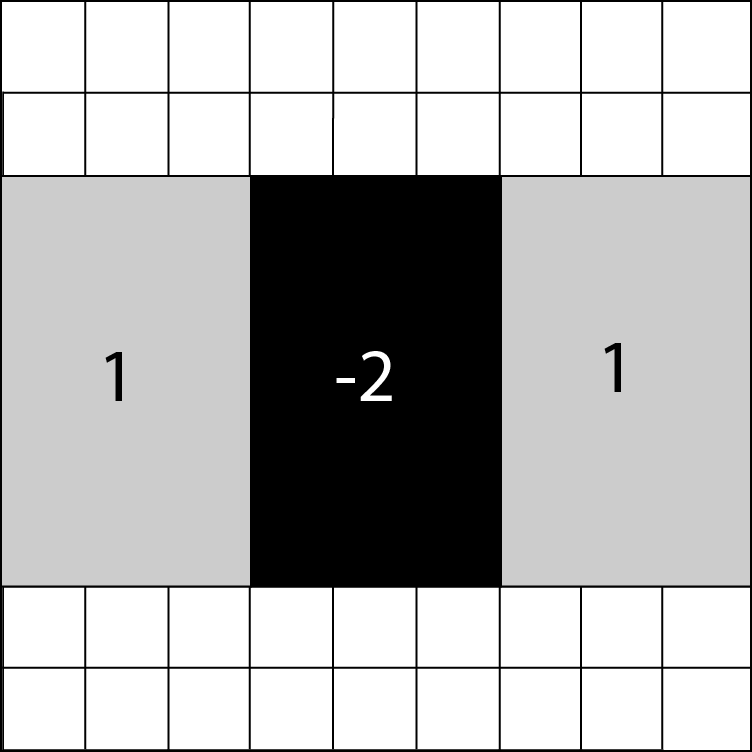
\includegraphics[width=\textwidth]{figures/hessian/gaussian_second_order_kernel_xx}
		\caption{$\frac{\partial^2 G}{\partial x_1^2}$}
	\end{subfigure}
	\begin{subfigure}[b]{0.3\textwidth}
		\centering
		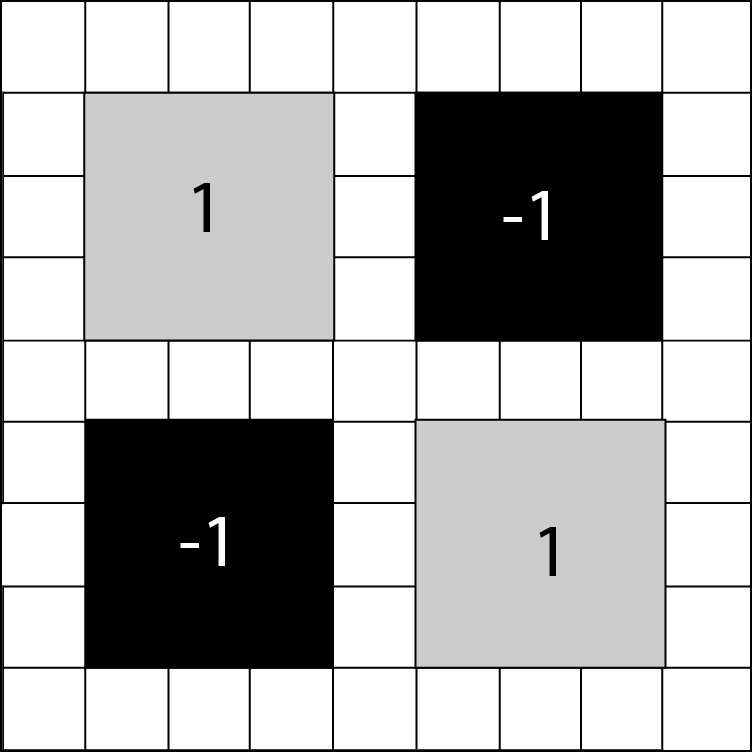
\includegraphics[width=\textwidth]{figures/hessian/gaussian_second_order_kernel_xy}
		\caption{$\frac{\partial^2 G}{\partial x_1 x_2}$}
	\end{subfigure}
	\begin{subfigure}[b]{0.3\textwidth}
		\centering
		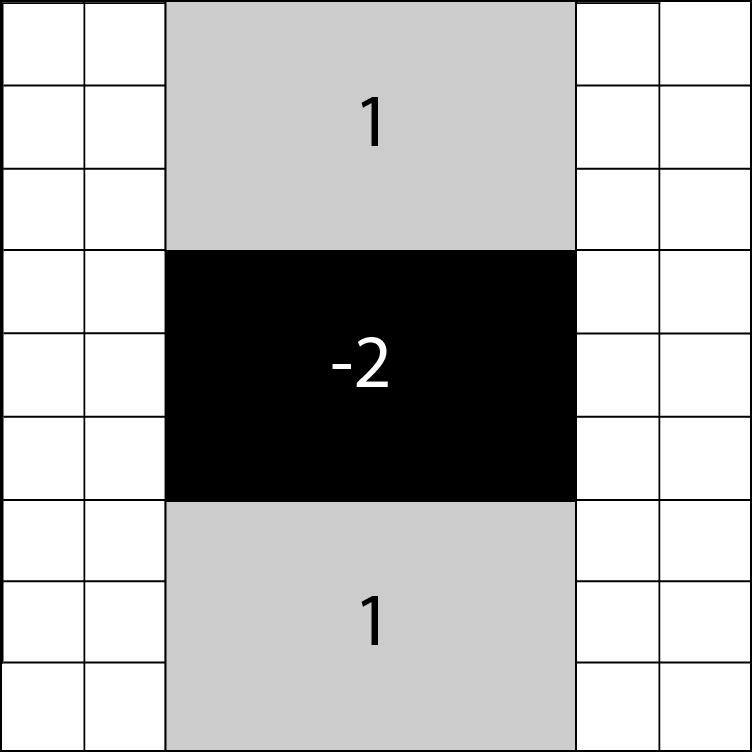
\includegraphics[width=\textwidth]{figures/hessian/gaussian_second_order_kernel_yy}
		\caption{$\frac{\partial^2 G}{\partial x_2^2}$}
	\end{subfigure}
	\caption{$9 \times 9$ discrete approximations of the Gaussian second order derivative with $\sigma=1.2$}
	\label{fig_gaussian_kernels}
\end{figure}

Another speed optimization presented in SURF takes advantage of the form of the discrete kernels. Since the approximated kernels are composed of rectangles of constant value, they can be decomposed into a set of box filters. Box filters can be computed quickly with the use of integral images. The general form of the integral image of an $M \times N$ image $I$ is shown in Equation \ref{eq_integral_image}.

\begin{equation}
\int I = \begin{bmatrix}
I(0,0) & \sum\limits_{m=0}^1 I(0,m) & \cdots & \sum\limits_{m=0}^M I(0,m) \\
\sum\limits_{n=0}^1 I(n,0) & \sum\limits_{n=0}^1 \sum\limits_{m=0}^1 I(n,m) & & \vdots \\
\vdots & & \ddots & \vdots \\
\sum\limits_{n=0}^N I(n,0) & \cdots & \cdots & \sum\limits_{n=0}^N \sum\limits_{m=0}^M I(n,m)
\end{bmatrix}
\label{eq_integral_image}
\end{equation}

Integral images decrease the computational complexity of finding the sum of an area in the input image. The computational complexity of strict kernel convolution at a point scales with the size of the kernel and is of the order $O(N^2)$ where the kernel is $N \times N$. A box filter can be decomposed into finding the sum of an area in the image and scaling it. Finding the sum from the integral image can be performed in $O(1)$ as shown in Equation \ref{eq_integral_image_box}. 

\begin{equation}
\sum\limits_{n=w}^y \sum\limits_{m=x}^z = \int I(y,z) - \int I(w-1,z) - \int I(y,x-1) + \int I(w-1, x-1)
\label{eq_integral_image_box}
\end{equation}

This makes the computation of the Hessian matrix scale only in terms of the image size, yielding no additional penalty for operating on different scale spaces.

\subsubsection{SURF Implementations for FPGA Devices}

The relatively low computational complexity makes SURF a popular choice for FPGA applications. Battezzati et al. present an architecture using accumulators for computing the integral image pipelined through the Hessian computation and storing detected feature points in a first in, first out (FIFO) cache \cite{battezzati_surf_2012}. These are matched against a stored set of feature points. Chen et al. present improvements on this approach by parallelizing the computation of different scale spaces \cite{chen_fpga-based_2016}. The implementation in this thesis follows these approaches with some additional improvements for speed based on the use case of matching against another image rather than a stored set of features.

\subsection{Iterative Closest Point Algorithm}

The crucial step in aligning the two images is the computation of an affine transform mapping one image into the space of the other. Once the images are aligned, they can be fused. A combination of SURF and the iterative closest point algorithm are used to compute this transform. Iterative closest point was first proposed by Chen and Medioni as a method for aligning 3-D point cloud data \cite{chen_object_1992}. In its simplest form, the algorithm follows the following steps:

\begin{enumerate}
	\item Each point in the set of points to be transformed is matched against the closest (usually Euclidean distance) point in the reference set of points.
	\item A transformation is estimated to minimize the distance between the transform set and their matches in the reference set of points.
	\item The transform is applied to the points.
\end{enumerate}

This process is repeated, converging to the local minimum that is the match between the two point sets.

Let $X_p(i)$ be be the $i^{th}$ point in the set of reference points onto which the transform points, $X(j)$, where $j$ is the index of the closest point to $X_p(i)$ in $X$, will be projected. The general form for this transformation $M$ is shown in Equation \ref{eq_general_icp_mapping}, and the expanded matrix form can be seen in Equation \ref{eq_expanded_icp_mapping}. In the expanded matrix form $M$ is decomposed into $R$, a $2 \times 2$ rotation matrix, and $T$, a translation offset.

\begin{equation}
X_p(i) = X(j) \cdot M
\label{eq_general_icp_mapping}
\end{equation}

\begin{equation}
\begin{bmatrix}
X_p(i)_1 \\
X_p(i)_2 \\
1 
\end{bmatrix}
=
\begin{bmatrix}
X(j)_1 & X(j)_2 & 1
\end{bmatrix}
\cdot
\begin{bmatrix}
R_{11} & R_{12} & T_1 \\
R_{21} & R_{22} & T_2 \\
0 & 0 & 1
\end{bmatrix}
\label{eq_expanded_icp_mapping}
\end{equation}

This equation only solves for $M$ for a single point relation, but can be restructured to contain
the whole set of $N$ points as shown in Equation \ref{eq_full_icp_matrix}. In this equation $P$ is a function $P: i \rightarrow j$ mapping the closest points in each set.

\begin{equation}
\begin{bmatrix}
X_p(0)_1 \\
X_p(0)_2 \\
X_p(1)_1 \\
X_p(1)_2 \\
\vdots \\
X_p(N)_1 \\
X_p(N)_2
\end{bmatrix}
=
\begin{bmatrix}
X(P(0))_1 & X(P(0))_2 & 1 & 0 & 0 & 0 \\
0 & 0 & 0 & X(P(0))_1 & X(P(0))_2 & 1 \\
X(P(1))_1 & X(P(1))_2 & 1 & 0 & 0 & 0 \\
0 & 0 & 0 & X(P(1))_1 & X(P(1))_2 & 1 \\
\vdots & & & & & \vdots \\
X(P(N))_1 & X(P(N))_2 & 1 & 0 & 0 & 0 \\
0 & 0 & 0 & X(P(N))_1 & X(P(N))_2 & 1 
\end{bmatrix}
\cdot
\begin{bmatrix}
R_{11} \\
R_{12} \\
T_1 \\
R_{21} \\
R_{22} \\
T_2
\end{bmatrix}
\label{eq_full_icp_matrix}
\end{equation}

Solving for $M$ in this way maps all points in $X$ to their closest points in $X_p$ based on an orthogonal projection with the error minimized in a least-squares sense. 

In this form, the transform $M$ will include shear transformations and non-uniform scaling. The computation can be simplified by forcing the second basis vector in $R$ to be orthogonal to the first. The two cameras are expected to be be physically in the same plane, and as such, non-uniform scaling and shear transformations are not expected for alignment. By setting $R_{21} = -R_{12}$ and $R_{22} = R{11}$, the computation of $M$ can be reduced as shown in Equation \ref{eq_reduced_icp_matrix}.

\begin{equation}
\begin{bmatrix}
X_p(0)_1 \\
X_p(0)_2 \\
X_p(1)_1 \\
X_p(1)_2 \\
\vdots \\
X_p(N)_1 \\
X_p(N)_2
\end{bmatrix}
=
\begin{bmatrix}
X(P(0))_1 & X(P(0))_2 & 1 & 0 \\
X(P(0))_2 & -X(P(0))_1 & 0 & 1 \\
X(P(1))_1 & X(P(1))_2 & 1 & 0 \\
X(P(1))_2 & -X(P(1))_1 & 0 & 1 \\
\vdots & & & \vdots \\
X(P(N))_1 & X(P(N))_2 & 1 & 0 \\
X(P(N))_2 & -X(P(N))_1 & 0 & 1 \\
\end{bmatrix}
\cdot
\begin{bmatrix}
R_{11} \\
R_{12} \\
T_1 \\
T_2
\end{bmatrix}
\label{eq_reduced_icp_matrix}
\end{equation}

If scaling is disallowed, and the transformation consists of only a translation and a rotation, this can be reduced further. Consider first computing the centroids of the point sets as in Equation \ref{eq_centroid}.

\begin{equation}
C = \frac{1}{N}\sum\limits_{i=1}^{N}X(i)
\label{eq_centroid}
\end{equation}

Based on the closest point matching, the covariance matrix $H$ can be computed as in Equation \ref{eq_covariance}.

\begin{equation}
H=\sum\limits_{i=1}^{N} (X(P(i)) - C) \cdot (X_p(i) - C_p)^T
\label{eq_covariance}
\end{equation}

The singular value decomposition $U\Sigma V = SVD(H)$ can be used to compute the rotation $R=VU^T$, where the translation is the distance between the centroids.

The performance of iterative closest point can be further improved by making it more sensitive to errors. Chetverikov introduced a variant of iterative closest point referred to as trimmed iterative closest point (TrICP) \cite{chetverikov_trimmed_2002}. TrICP is more robust to errors by eliminating points that introduce error into the matching. Some detected features points will not have correspondences between images. By eliminating these points, the overall error can be reduced to compute a more accurate transform.

\subsection{Singular Value Decomposition (SVD)}

Let Equation \ref{eq_reduced_icp_matrix} be of the form $X=Q \cdot M$. In order to compute the transform $M$, the equation must be restructured as in Equation \ref{eq_svd_inverse}.

\begin{equation}
Q^{-1} X = M
\label{eq_svd_inverse}
\end{equation}

$Q$ is not a square matrix, and as such is not invertible, but its pseudoinverse can be used in this instance. The pseudoinverse is computed through the use of singular value decomposition. The use of singular value decomposition to compute the transform is the source of the least squares fitting achieved by iterative closest point.

This is necessary for computing transforms with more degrees of freedom, however for rigid body transformations, it is sufficient to find the singular value decomposition of the covariance matrix $H$, a $2 \times 2$ matrix for which a closed form solution does exist\cite{blinn_consider_1996} and is shown in Equation \ref{eq_svd_decomp}.

\begin{equation}
\begin{gathered}
	\begin{bmatrix}
	A & B \\
	C & D
	\end{bmatrix}
	=
	\begin{bmatrix}
	cos\beta & sin\beta \\
	-sin\beta & cos\beta
	\end{bmatrix}
	\begin{bmatrix}
	w_1 & 0 \\
	0 & w_2
	\end{bmatrix}
	\begin{bmatrix}
	cos\gamma & sin\gamma \\
	-sin\gamma & cos\gamma
	\end{bmatrix}
	=
	\begin{bmatrix}
	E & H \\
	-H & E
	\end{bmatrix}
	+
	\begin{bmatrix}
	F & G \\
	G & -F
	\end{bmatrix}
	\\
	\frac{w_1 + w_2}{2} = \sqrt{E^2 + H^2}
	\\
	\frac{w_1 - w_2}{2} = \sqrt{F^2 + G^2}
	\\
	\gamma - \beta = tan^{-1}(G/F)
	\\
	\gamma + \beta = tan^{-1}(H/E)
\end{gathered}
\label{eq_svd_decomp}
\end{equation}

\subsubsection{SVD Implementations for FPGA Devices}

Singular value decomposition can be performed on FPGAs by cascading a set of $2 \times 2$ cells \cite{wang_singular_2010}. Ledesma-Carillo et al. present a hardware efficient algorithm for computing singular value decompositions on large matrices using one-sided Jacobi rotations for computing SVD on arbitrary $M \times N$ matrices \cite{ledesma-carrillo_reconfigurable_2011}. One of these approaches is necessary if the sensor fusion must correct for scale or shear. It is worth noting that these approaches both require very high utilization of the FPGA, and as such may be difficult to implement for large numbers of feature points.

In contrast, if only a rigid body transformation is required, then Equation \ref{eq_svd_decomp} can be implemented trivially using CORDIC approximations for the square root and arctangent functions.

\section{Implementation}

The implementation of this design was performed on a ZedBoard Zynq-7000 ARM/FPGA SoC Development Board.

\subsection{Camera Interface}

The design was implemented using a pair of OV7670 VGA cameras. These cameras feature an $I^2C$ interface for configuration, and generate hsync and vsync VGA timing signals along with 8 bits of data. They can be configured to output 16-bit RGB(565) with half of the RGB signal sent on each clock pulse. Configured this way, the camera outputs a resolution of $640$ by $480$ pixels at $30Hz$. 

\subsection{Streaming Kernel Operators}

Performing kernel convolution in real time is complicated by the fact that a pixel has data dependencies on its neighbors. As such, the input data must be buffered until all of the necessary data is available to perform convolution at a given point. The buffer size must be at least $N \times W + M$ where the kernel is $M \times N$ and the image is of width $W$. On FPGAs, this minimally sized buffer can be implemented using LUTRAM, a hardware lookup table. LUTRAM on most FPGAs also has the advantage of being able to act as a set of shift registers. The convolution multipliers and adders can be attached to a single set of cells, and the data can be shifted through the array as it streams. The architecture for this scan chain approach for computing $3 \times 3$ kernel convolution can be seen in Figure \ref{fig_block_scanchain}.

\begin{figure}[h]
	\centering
	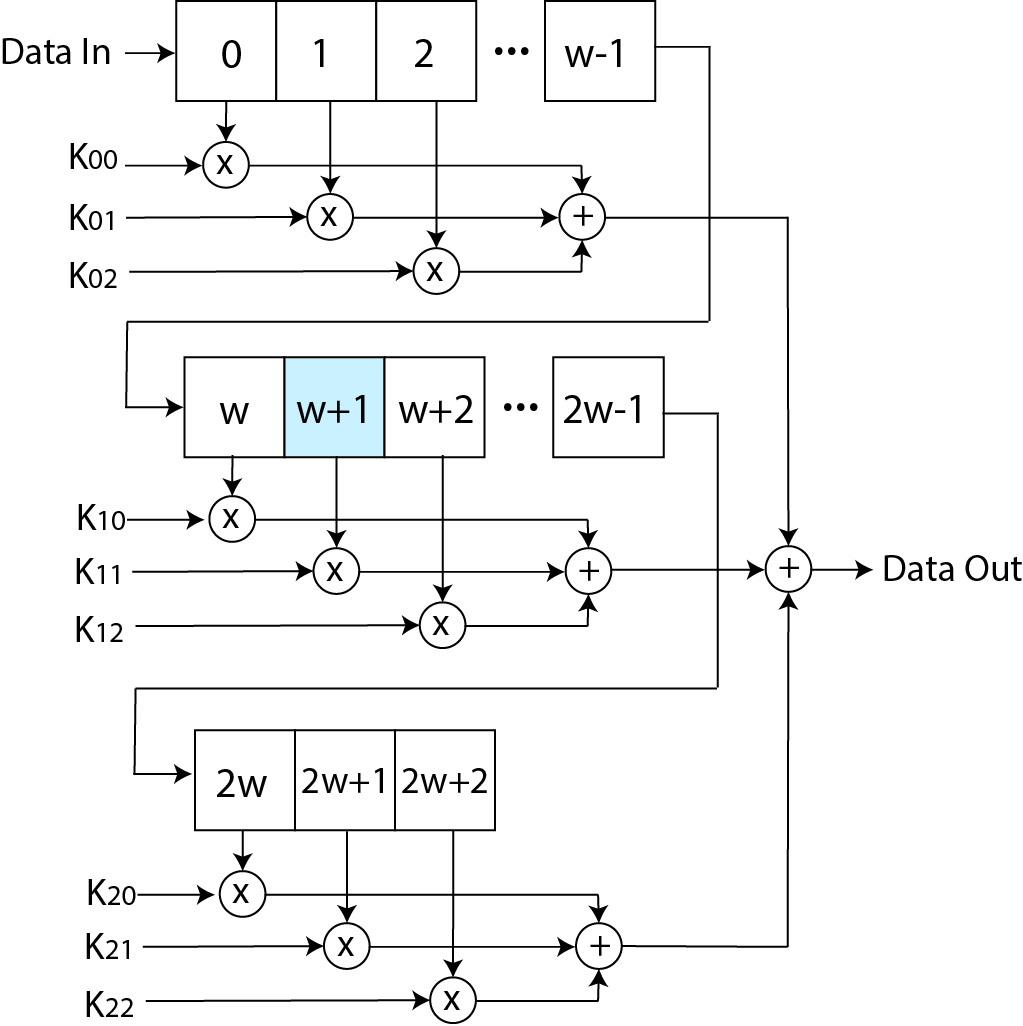
\includegraphics[width=0.6\textwidth]{figures/block/scanchain}
	\caption{Block diagram for computing $3 \times 3$ kernel convolution on a data stream using a scan chain}
	\label{fig_block_scanchain}
\end{figure}

This scan chain approach to kernel convolution is the faster and more utilization efficient approach to performing kernel convolution on streamed data. However, LUTRAM on most FPGAs is a limited resource, and as such, large kernels and image widths will make it difficult to implement a design. Implementing an LUTRAM scan chain for performing operations on $9 \times 9$ kernels with an image width of $640$ pixels on the Xilinx Zynq XC7Z020-1CLG484 chipset used for this design consumed $96\%$ of the available LUTRAM. Since it was necessary to implement two hessian operators, one for each camera, an approach was devised to utilize the slower, but more plentiful block RAM.

The block RAM has limitations. The data cells inside of the block RAM are not directly accessible. They must be read or written by writing an address to a control port and then waiting for the designated latency. The process of reading and writing to and from block RAM can be pipelined, that is, instructions can be given in sequence and then after the initial latency, data will be read and written every clock cycle. This will be explored in more detail in the design of the Hessian kernel operator.

\subsubsection{Hessian Kernel Operators}

The kernels discussed in this section are the $9 \times 9$ discrete approximations shown in Figure \ref{fig_gaussian_kernels}. If straightforward kernel convolution were to be implemented, it would require sampling all points with non-zero kernel values which would not be realistic for performing these operators in real time. Instead, the integral image is used to reduce the number of required sampling points. Recall that the integral image can be used to compute the area in a rectangle by sampling the corners, adding the bottom-right corner and top-left corner, and subtracting the bottom-left corner and top-right corner. As such, the required sampling points for the SURF kernels are highlighted in Figure \ref{fig_gaussian_integral_kernels}.

\begin{figure}[h]
	\centering
	\begin{subfigure}[b]{0.3\textwidth}
		\centering
		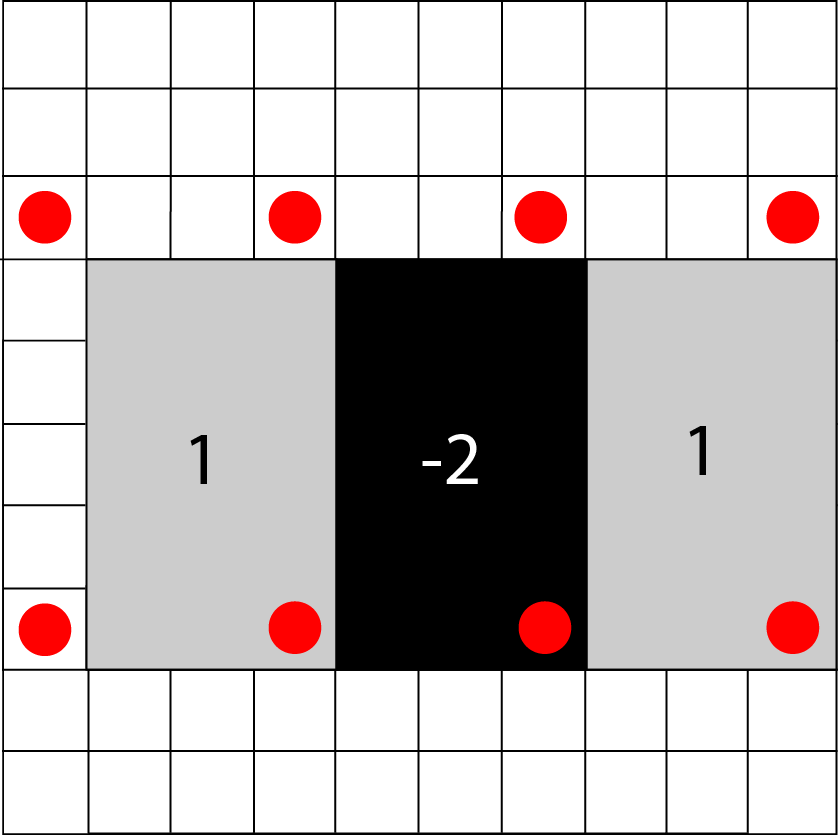
\includegraphics[width=\textwidth]{figures/hessian/gaussian_second_order_kernel_xx_integral}
		\caption{$\frac{\partial^2 G}{\partial x_1^2}$}
	\end{subfigure}
	\begin{subfigure}[b]{0.3\textwidth}
		\centering
		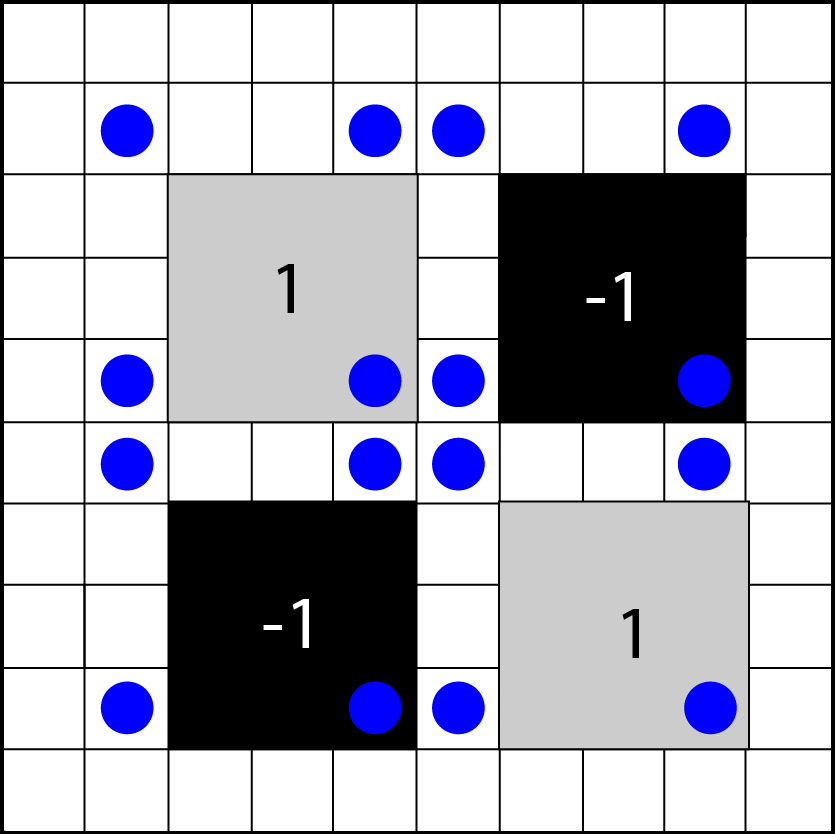
\includegraphics[width=\textwidth]{figures/hessian/gaussian_second_order_kernel_xy_integral}
		\caption{$\frac{\partial^2 G}{\partial x_1 x_2}$}
	\end{subfigure}
	\begin{subfigure}[b]{0.3\textwidth}
		\centering
		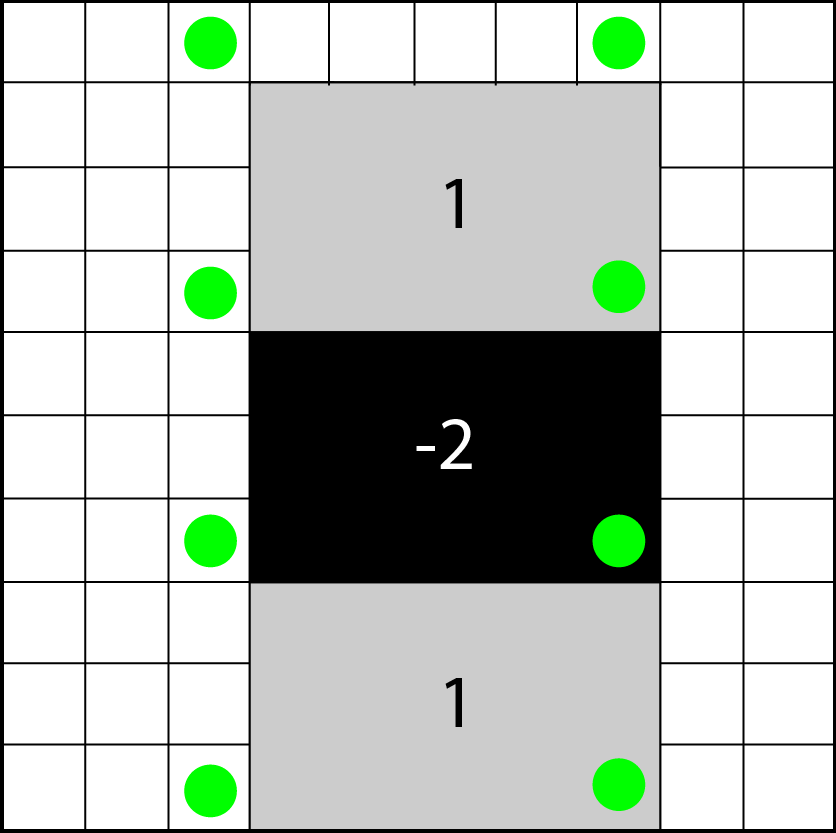
\includegraphics[width=\textwidth]{figures/hessian/gaussian_second_order_kernel_yy_integral}
		\caption{$\frac{\partial^2 G}{\partial x_2^2}$}
	\end{subfigure}
	\caption{$9 \times 9$ SURF kernels with marked integral sampling points}
	\label{fig_gaussian_integral_kernels}
\end{figure}

It can be observed in Figure \ref{fig_gaussian_integral_kernels} that the worst-case for the data dependencies is the bottom-right point in $\frac{\partial^2 G}{\partial x_2^2}$. If the Hessian determinant is to be computed with minimal latency, it should be computed when that point becomes available. In order to compute the integral at a point, the integral above, to the left, and to the top-left of the desired point must be sampled. From this, it can be concluded that thirty-four points must be sampled to compute the Hessian determinant (eight from $\frac{\partial^2 G}{\partial x_1^2}$, sixteen from $\frac{\partial^2 G}{\partial x_1 x_2}$, seven from $\frac{\partial^2 G}{\partial x_2^2}$, and three to compute the integral). 

In order to do this in real time, the Hessian determinant must be computable within a pixel clock cycle. Given a resolution of $640$ by $480$ at $30$ frames per second, this is a pixel clock speed of $12.5 MHz$. Recall that block RAM must be addressed and read. In this implementation, block RAM has a latency of three clock cycles. In order to compute the determinant in a single pixel clock cycle, the Hessian block is clocked at $200 Mhz$, giving it $16$ clock cycles for every pixel clock cycle. A $200 Mhz$ clock has a period of only $5ns$ which makes pipelining of instructions very important in order to meet timing. A dual port block RAM was used, with addressing using the lower bits of $y$ to map into a modular address space of $16$ rows. The dual port RAM effectively allows for $32$ read/write operations within the pixel clock period. An LUTRAM cache containing the integral values for the last row up to the top-left point required for the integral image reduces the number of memory reads for required points to $29$, along with a single memory write to place the last value in the cache into the block RAM. The set of pipeline instructions for computing the Hessian determinants can be found in Tables \ref{table_pipeline_1}, \ref{table_pipeline_2}, and \ref{table_pipeline_3}. In these tables, $L$ represents the rectangles that make up the SURF kernels. Its subscripts, such as $L_{xx_n}$ refer to the specific rectangle. $L_{xx}$ is numbered from right to left, $L_{xy}$ is numbered clockwise beginning at the top left, and $L_{yy}$ is numbered from top to bottom referring to what is shown in Figure \ref{fig_gaussian_integral_kernels}.

\begin{table}[h]
	\centering
	\caption{Stages 1-8 of pipeline instructions for computing Hessian determinants}
	\label{table_pipeline_1}
	\begin{tabulary}{1.0\textwidth}{L|L|L}
		Cycle & Instruction \#1 & Instruction \#2 \\
		\hline
		
		1. & $\bullet$ Store current (x,y) and value in registers & $\bullet$ Get integral top, left, and corner from cache \\
		& & $\bullet$ Compute top left and top right addresses for $L_{yy_2}/L_{yy_1}$ \\
		& & $\bullet$ Write addresses to read top left and top right of $L_{yy_1}/L_{yy_0}$ \\
		& & $\bullet$ Data ready, bottom right and top right corner of $L_{xx_2}/L_{xx_1}$ \\
		& & $\bullet$ Compute $L_{xx_0}$ \\
		\hline
		
		2. & $\bullet$ Compute (x,y) bottom right and top left corner for $L_{xy_0}$ & $\bullet$ Write addresses to read top left and top right corner of $L_{yy_2}/L_{yy_1}$ \\
		& & $\bullet$ Data ready, bottom left and top left corner of $L_{xx_2}$ \\
		& & $\bullet$ Compute $L_{xx_1}$ \\
		& & $\bullet$ Compute integral \\
		\hline
		
		3. & $\bullet$ Compute (x,y) bottom left and top right corner for $L_{xy_0}$ & $\bullet$ Data ready, top left and top right corner for $L_{yy_0}$ \\
		& Compute bottom right and top left addresses for $L_{xy_0}$ & $\bullet$ Compute $L_{xx_2}$ \\
		\hline
		
		4. & $\bullet$ Compute (x,y) bottom right and top left corner for $L_{xy_1}$ & $\bullet$ Data ready, top left and top right corner of $L_{yy_1}/L_{yy_0}$ \\
		& $\bullet$ Compute bottom left and top right addresses for $L_{xy_0}$ & $\bullet$ Compute $L_{xx}$ \\
		& $\bullet$ Write addresses to read bottom right and top left of $L_{xy_0}$ & \\
		\hline
		
		5. & $\bullet$ Compute (x,y) bottom left and top right corner for $L_{xy_1}$ & $\bullet$ Data ready, top left and top right corner of $L_{yy_2}/L_{yy_1}$ \\
		& $\bullet$ Compute bottom right and top left addresses for $L_{xy_1}$ & $\bullet$ Compute $L_{yy_0}$ \\
		& $\bullet$ Write addresses to read bottom left and top right of $L_{xy_0}$ & \\
		\hline
		
		6. & $\bullet$ Compute (x,y) bottom right and top left corner for $L_{xy_2}$ & $\bullet$ Compute $L_{yy_1}$ \\
		& $\bullet$ Compute bottom left and top right addresses for $L_{xy_1}$ & \\
		& $\bullet$ Write addresses to read bottom right and top left of $L_{xy_1}$ & \\
		\hline 
		
		7. & $\bullet$ Compute (x,y) bottom left and top right corner for $L_{xy_2}$ & $\bullet$ Compute $L_{yy_2}$ \\
		& $\bullet$ Compute above point address for write & \\
		& $\bullet$ Compute top left address for $L_{xy_2}$ & \\
		& $\bullet$ Write addresses to read bottom left and top right of $L_{xy_1}$ & \\
		& $\bullet$ Data ready, bottom right and top left corner of $L_{xy_0}$ & \\
		\hline
		
		8. & $\bullet$ Compute (x,y) bottom right and top left corner for $L_{xy_3}$ & $\bullet$ Shift cache \\
		& $\bullet$ Compute bottom left and top right addresses for $L_{xy_2}$ & $\bullet$ Compute $L_{yy}$ \\
		& $\bullet$ Write addresses to write above point and read top left corner of $L_{xy_2}$ & \\
		& $\bullet$ Data ready, bottom left and top right corner of $L_{xy_0}$ & \\
		\hline
	\end{tabulary}
\end{table}

\begin{table}[h]
	\centering
	\caption{Stages 9-13 of pipeline instructions for computing Hessian determinants}
	\label{table_pipeline_2}
	\begin{tabulary}{1.0\textwidth}{L|L|L}
		\hline
		9. & $\bullet$ Compute (x,y) bottom left and top right corner for $L_{xy_3}$ & \\
		& $\bullet$ Compute bottom right and top left addresses for $L_{xy_3}$ & \\
		& $\bullet$ Write addresses to read bottom left and right of $L_{xy_2}$ & \\
		& $\bullet$ Data ready, bottom right and top left corner of $L_{xy_1}$ & \\
		& $\bullet$ Compute $L_{xy_0}$ & \\
		\hline
		
		10. & $\bullet$ Compute (x,y) bottom right and top right for $L_{xx_0}$ & $\bullet$ Compute determinant secondary diagonal \\
		& $\bullet$ Compute bottom left and top right addresses for $L_{xy_3}$ & \\
		& $\bullet$ Write addresses to read bottom right and top left of $L_{xy_3}$ & \\
		& $\bullet$ Data ready, bottom left and top right corner of $L_{xy_1}$ & \\
		\hline
		
		11. & $\bullet$ Compute (x,y) bottom right and top right for $L_{xx_1}/L_{xx_0}$ & \\
		& $\bullet$ Compute bottom right and top right addresses for $L_{xx_0}$ & \\
		& $\bullet$ Write addresses to read bottom left and top right of $L_{xy_3}$ & \\
		& $\bullet$ Data ready, bottom right and top left corner of $L_{xy_2}$ & \\
		& $\bullet$ Compute $L_{xy_1}$ & \\
		\hline
		
		12. & $\bullet$ Compute (x,y) bottom right and top left for $L_{xx_2}/L_{xx_1}$ & \\
		& $\bullet$ Compute bottom right and top right addresses for $L_{xx_1}/L_{xx_0}$ & \\
		& $\bullet$ Write addresses to read bottom right and top right for $L_{xx_0}$ & \\
		& $\bullet$ Data ready, bottom left and top right corner of $L_{xy_2}$ & \\
		\hline
		
		13. & $\bullet$ Compute (x,y) bottom left and top left for $L_{xx_2}$ & $\bullet$ Compute determinant primary diagonal \\
		& $\bullet$ Compute bottom right and top right addresses for $L_{xx_2}/L_{xx_1}$ & \\
		& $\bullet$ Write addresses to read bottom right and top right of $L_{xx_1}/L_{xx_0}$ & \\
		& $\bullet$ Data ready, bottom right and top left corner of $L_{xy_3}$ & \\
		& $\bullet$ Compute $L_{xy_2}$ & \\
		\hline
	\end{tabulary}
\end{table}
		
\begin{table}[h]
	\centering
	\caption{Stages 14-16 of pipeline instructions for computing Hessian determinants}
	\label{table_pipeline_3}
	\begin{tabulary}{1.0\textwidth}{L|L|L}
		\hline
		14. & $\bullet$ Compute (x,y) top left and top right for $L_{yy_0}$ & $\bullet$ Compute determinant \\
		& $\bullet$ Compute bottom left and top left addresses for $L_{xx_2}$ & \\
		& $\bullet$ Write addresses to read bottom right and top right of $L_{xx_2}/L_{xx_1}$ & \\
		& $\bullet$ Data ready, bottom left and top right corner of $L_{xy_3}$ & \\
		\hline
		
		15. & $\bullet$ Compute (x,y) top left and top right for $L_{yy_1}/L_{yy_0}$ & $\bullet$ Absolute value determinant \\
		& $\bullet$ Compute top left and top right addresses for $L_{yy_0}$ & \\
		& $\bullet$ Write addresses to read bottom left and top left of $L_{xx_2}$ & \\
		& $\bullet$ Data ready, bottom right and top right corner of $L_{xx_0}$ & \\
		& $\bullet$ Compute $L_{xy_3}$ & \\
		\hline
		
		16. & $\bullet$ Compute (x,y) top left and top right for $L_{yy_2}/L_{yy_1}$ & $\bullet$ Write determinant \\
		& $\bullet$ Compute top left and top right addresses for $L_{yy_1}/L_{yy_0}$ & \\
		& $\bullet$ Write addresses to read top left and top right corner of $L_{yy_0}$ & \\
		& $\bullet$ Compute $L_{xy}$ & \\
	\end{tabulary}
\end{table}

When computed in this way, the Hessian determinant at a point will be outputted at the end of the next pixel clock cycle continuously as the data stream passes through the system. It is worth noting that this implementation does not need to be modified to compute Hessian determinants in different scale spaces. Larger kernels still have the same number of points that must be sampled, but the required block RAM for the design does grow with the kernel size.

\subsubsection{Average Filter Approximation of Single Level Laplacian Pyramid}

In this design, only a single level of the Laplacian pyramid is used for fusion. In a single level, a Gaussian blur is applied to the image. It is downsampled, upsampled, and subtracted from the original. The downsampling and upsampling in a single level can be approximated as an average filter without performing the costly operation of modifying the resolution of the image. In this design, the Gaussian and average filters were implemented as a set of scan chains to perform $3 \times 3$ kernel convolution.

\subsubsection{Application of Non-maximum Suppression}

Though not a kernel operator, non-maximum suppression depends on the data points around it. Non-maximum suppression is to be applied to the Hessian determinant values in order to reduce them to a smaller, more precise set of features. In a $3$ by $3$ neighborhood, if the central pixel is not the maximum, it is set to zero. In this way, only the peak features remain for processing. The $3x3$ neighborhood search was implemented as a $3 \times 3$ scan chain with comparison operators.

\subsection{Computation of Transform from Detected Features}

As features are generated, they are passed into a feature buffer as a tuple of their magnitude, x, and y coordinates. The buffer is made up of bubble-sort cells as shown in Figure \ref{fig_bubblesort}.

\begin{figure}[h]
	\centering
	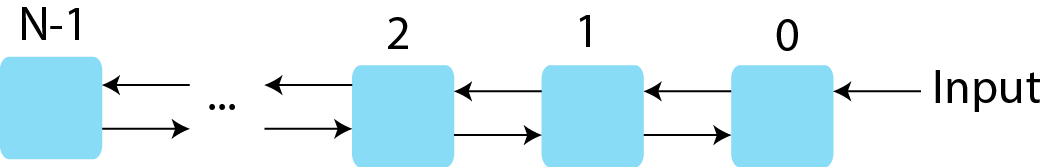
\includegraphics[width=0.8\textwidth]{figures/block/bubblesort}
	\caption{Bubble-sort architecture of the feature buffer}
	\label{fig_bubblesort}
\end{figure}

On the rising edge of the clock, the even cells swap values with their neighbor to the left if the cell contains a greater value than its neighbor. On the falling edge, the odd cells do the same. In this way, the highest valued elements propagate to the top of the buffer, and lower valued elements are dropped out of the bottom. The comparison criteria for this operation is the Hessian magnitude, and the sort is active for as long as features are being generated. At the end of the frame, the buffer contains only the points with the highest Hessian magnitudes.

Once the points have been collected, the transform set is compared to the reference set and correspondences are assigned based on euclidean distance to find the closest point. This is done via a brute-force search. Every point is compared to every other, and the closest one emerges. The architecture of this comparison is shown in Figure \ref{fig_comparison}.

\begin{figure}[h]
	\centering
	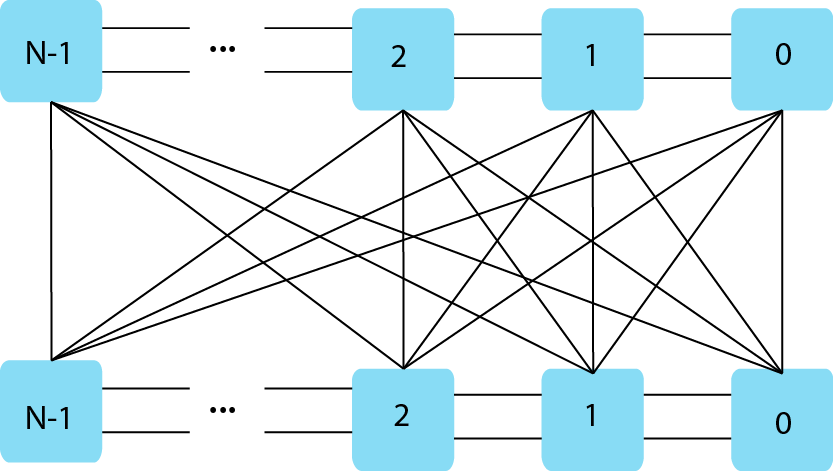
\includegraphics[width=0.8\textwidth]{figures/block/comparison}
	\caption{Feature buffer brute-force comparison}
	\label{fig_comparison}
\end{figure}

For low numbers of feature points, the inefficiency of brute-force search is mitigated by its simplicity. In hardware, a brute force comparison like this does not suffer from additional time complexity since the comparisons all happen in parallel. However, the space complexity and fanout of the circuit goes up exponentially as more cells are added.

It should be intuitive that this architecture is only useful for small numbers of feature points. The high fanout of the brute force comparison quickly becomes unmanageable to route in most designs with more than a handful of features. In the case that this becomes difficult, it is possible to trade the space complexity of the design for time complexity by making the computation iterative as in Figure \ref{fig_comparison_iter}.

\begin{figure}[h]
	\centering
	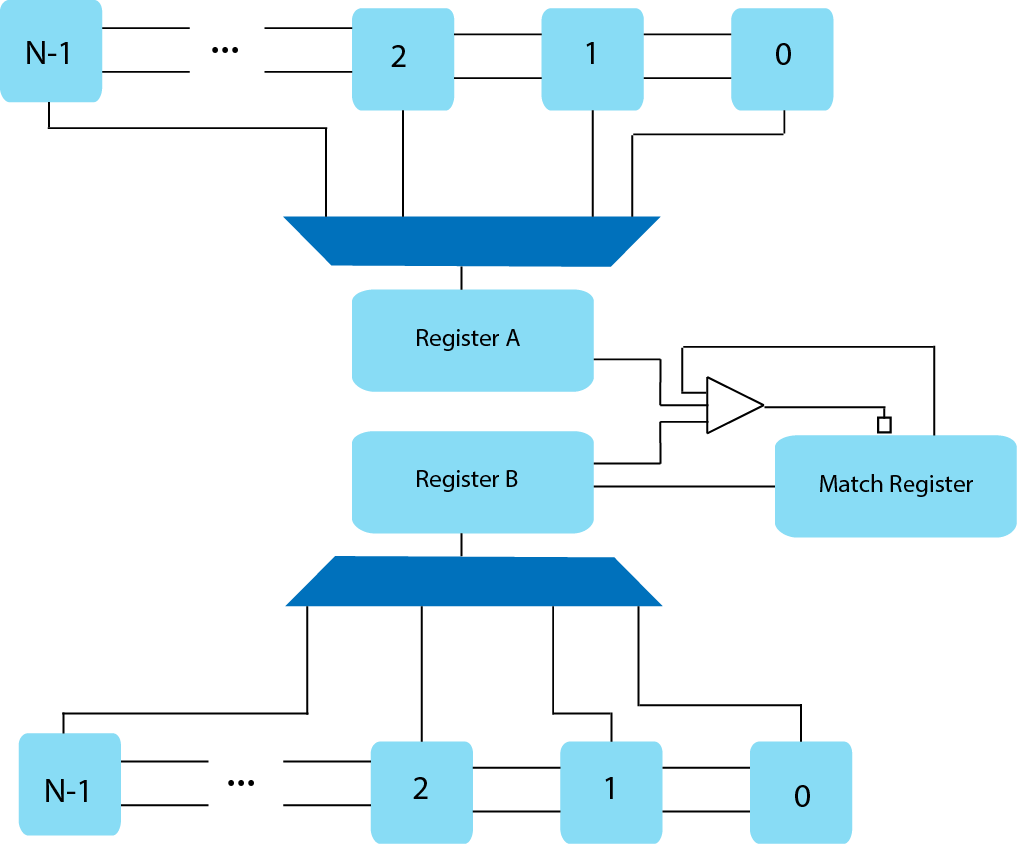
\includegraphics[width=0.8\textwidth]{figures/block/comparison_iter}
	\caption{Feature buffer iterative comparison}
	\label{fig_comparison_iter}
\end{figure}

In this approach, the a point from the reference set is loaded into register A. Then, each point in the transform set is loaded into register B in turn. If the distance between the loaded value and the value in register A is less than the distance between the value stored in the match register and register A, then the loaded value from register B is placed into the match register. This is repeated for all elements in the reference set to find their closest points in the transform set.

\subsection{Application of Transform to Real-Time Data}

The transform is applied through the use of a frame buffer. The reference image remains fixed and is outputted as normal. However, the address for the transform image is decomposed into x and y coordinates. This is multiplied through the computed transform, and the transformed coordinates are used to select pixels from the frame buffer. The reference pixel and transform pixel are then fused together to create the output stream.

The transform is recomputed at the end of the frame from the detected features and then applied to the next generation of incoming data. In this way, the transform is additively refined as in iterative closest point. The transform computed for a frame is concatenated with the transform from the last frame, eventually converging to a local error minimum for alignment in a least squares sense. 

\section{Results}

\subsection{Detecting feature points in real time}

The system for detecting feature points in real time is demonstrated through a picture of the system output shown in Figure \ref{fig_pic_features}. Detected feature points above a threshold are marked in white, showing the detection of strong changes in gradient, particularly evident around the eyes and nose.

\begin{figure}[h]
	\centering
	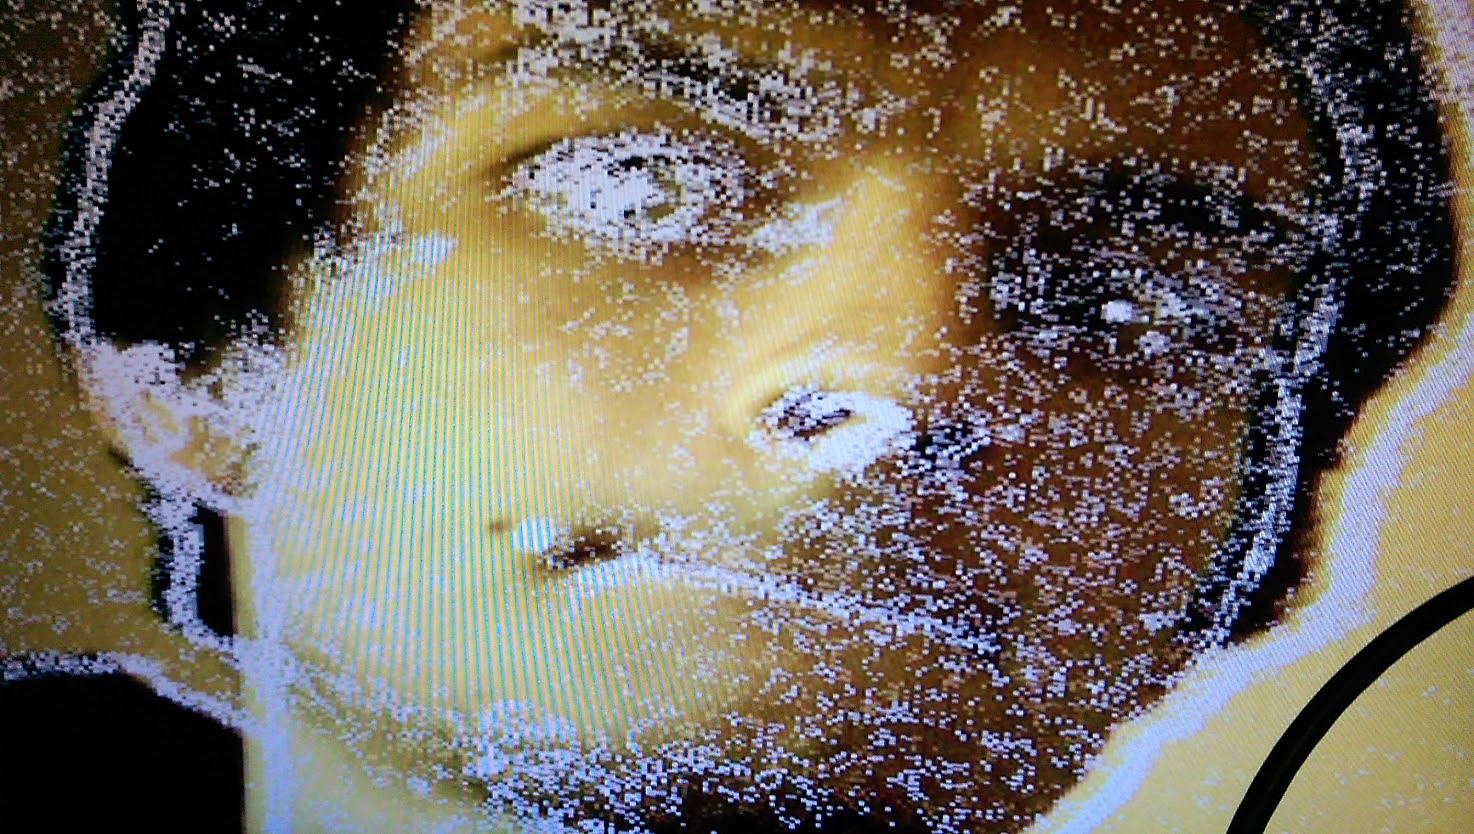
\includegraphics[width=0.8\textwidth]{figures/pictures/features}
	\caption{Real-time capture of Hessian feature points}
	\label{fig_pic_features}
\end{figure}

\subsection{Selecting an optimal number of feature points}

A set of experiments to align the images shown in Figure \ref{fig_waterboy_left_right} were performed using different numbers of feature points for a variable number of iterations of the iterative closest point algorithm.

The iterative closest point algorithm always converges to a solution which minimizes the overall distance between the transform and reference set of points. This can be observed in Figure \ref{fig_results_error_plot} which shows the average distance from each point in the transform set of points to its closest neighbor in the reference set of points. Regardless of the selected number of features, all experiments converge to a roughly the same minimum. However, this may be an optimal solution in terms of distances between the feature points, but it is not always optimal in terms of alignment. 

\begin{figure}
	\centering
	\begin{subfigure}[b]{0.3\textwidth}
		\centering
		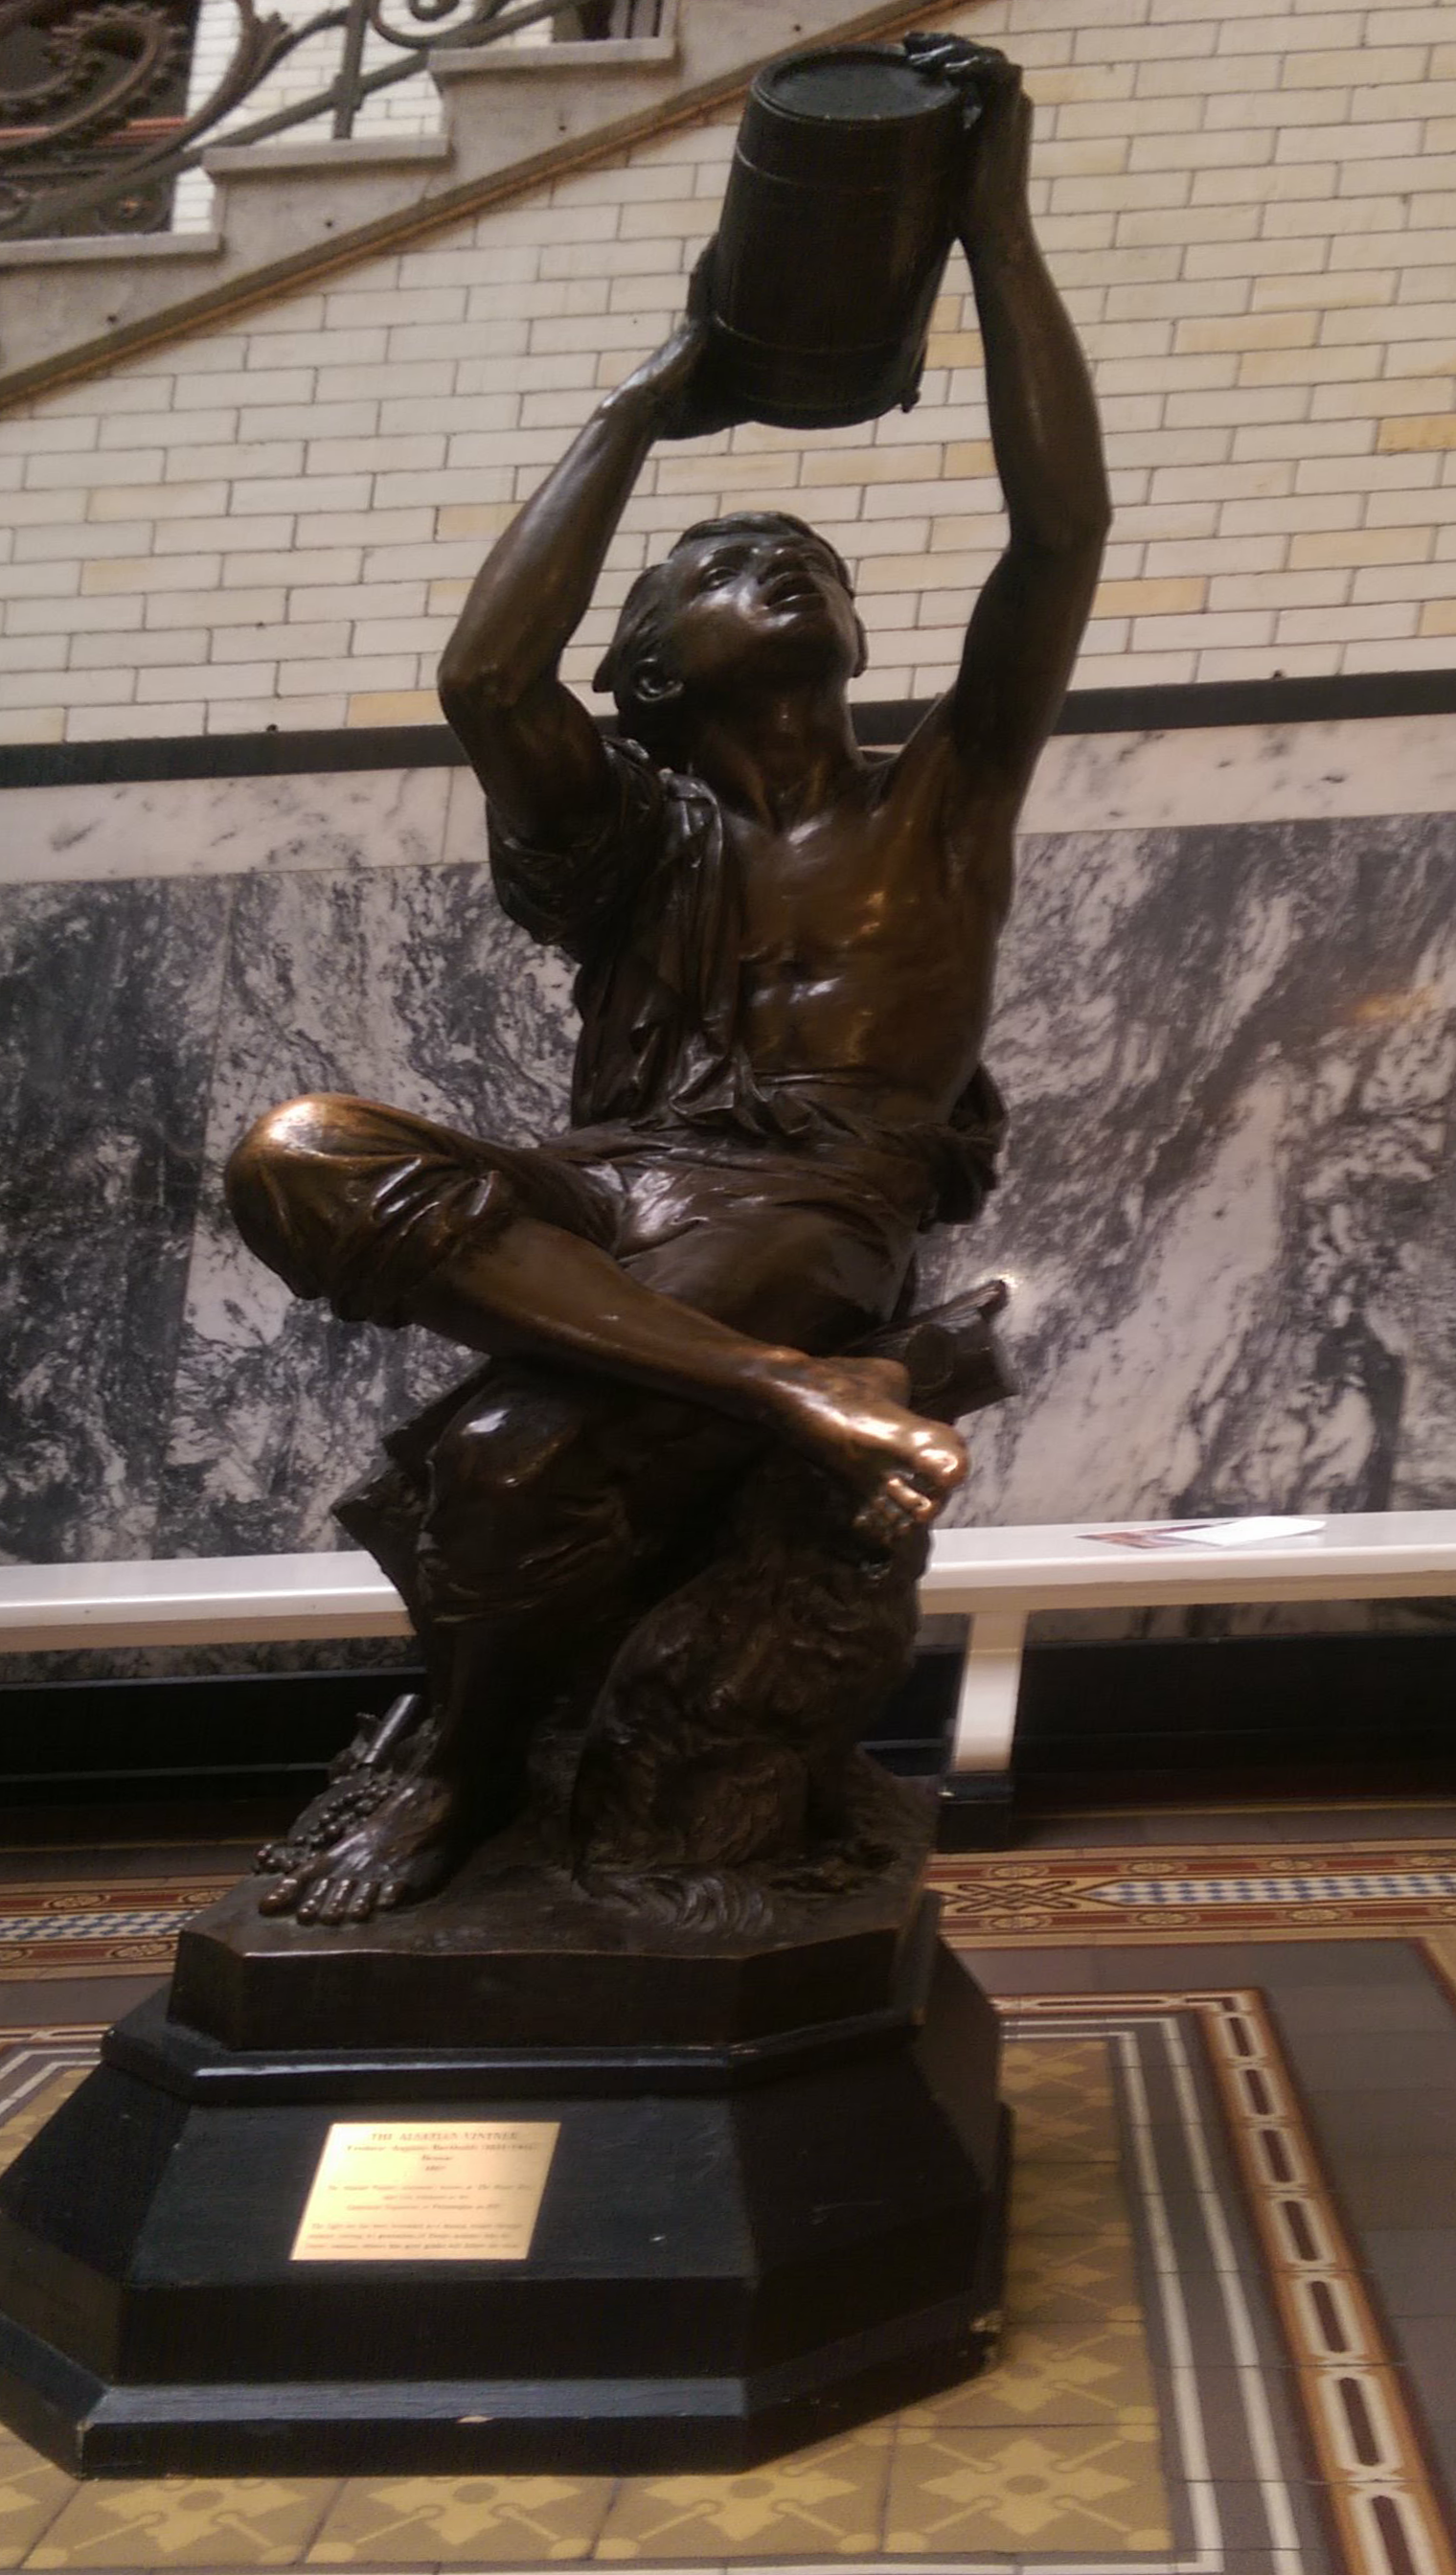
\includegraphics[width=\textwidth]{figures/alignment/waterboy_left}
		\caption{Reference Image}
	\end{subfigure}
	\begin{subfigure}[b]{0.3\textwidth}
		\centering
		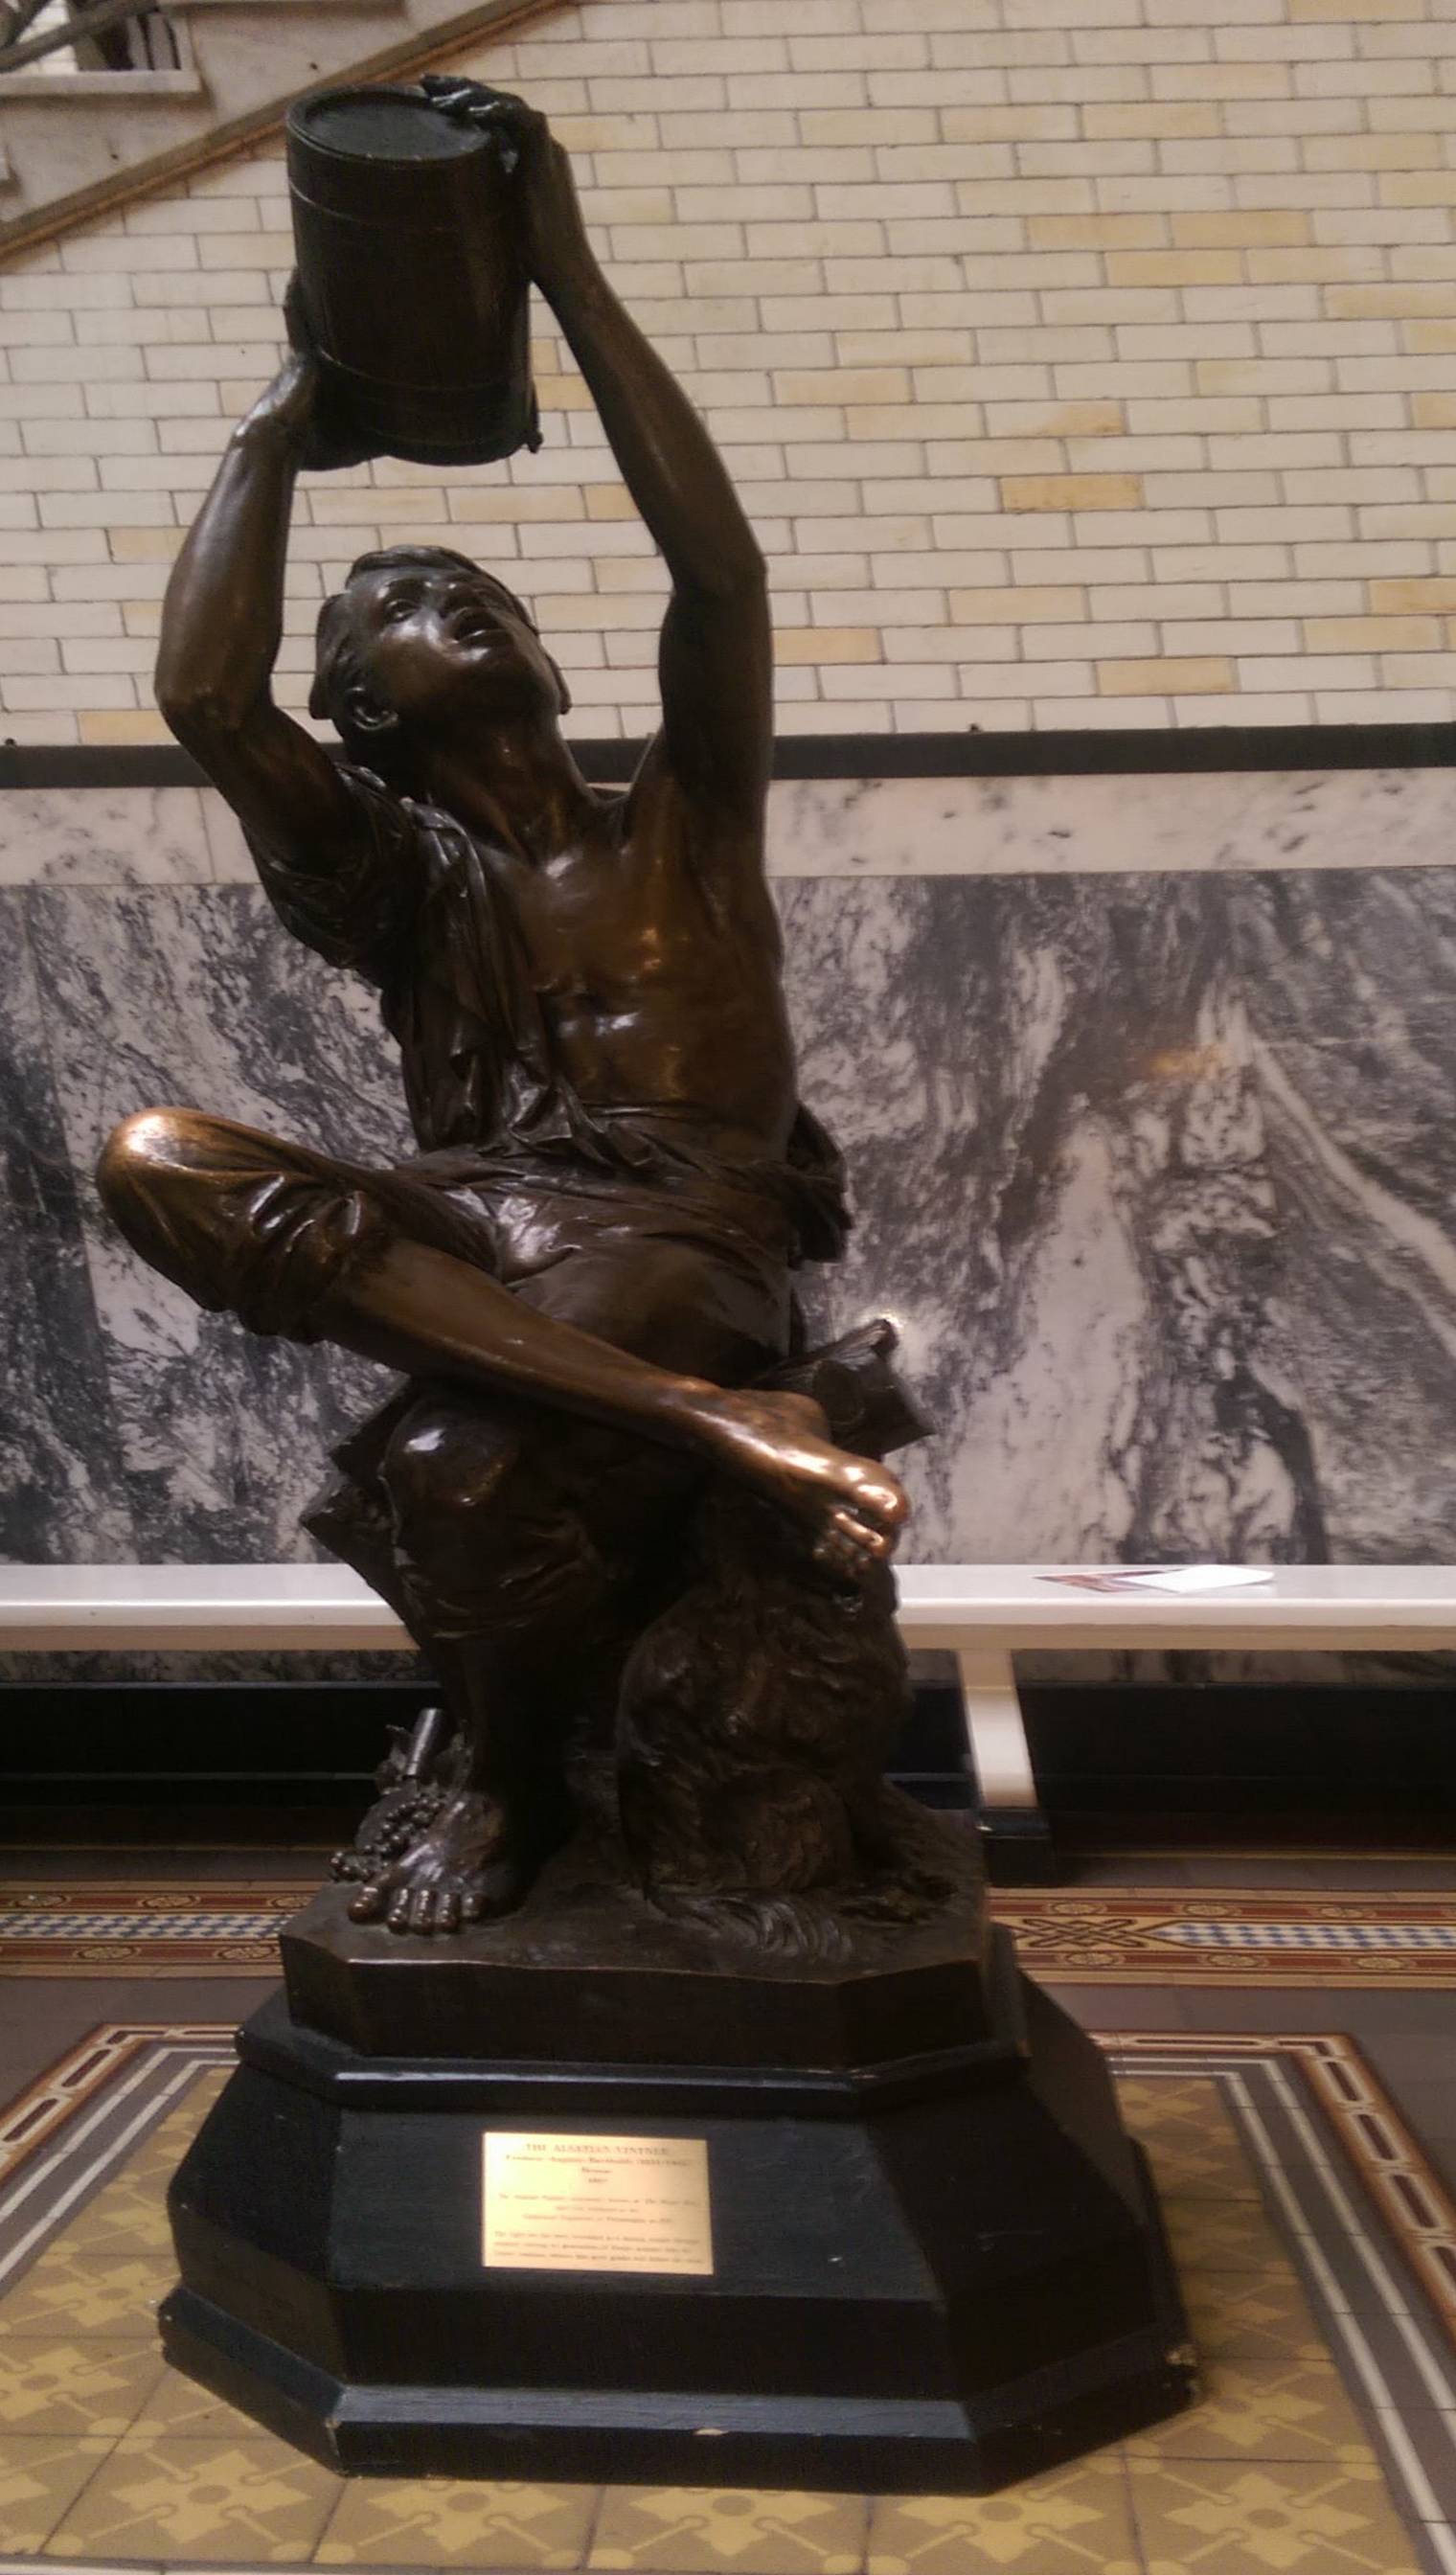
\includegraphics[width=\textwidth]{figures/alignment/waterboy_right}
		\caption{Transform Image}
	\end{subfigure}
	\caption{Images of "The Water Boy" by Frédéric-August Bartholdi from the Drexel Collection}
	\label{fig_waterboy_left_right}
\end{figure}

\begin{figure}[h]
	\centering
	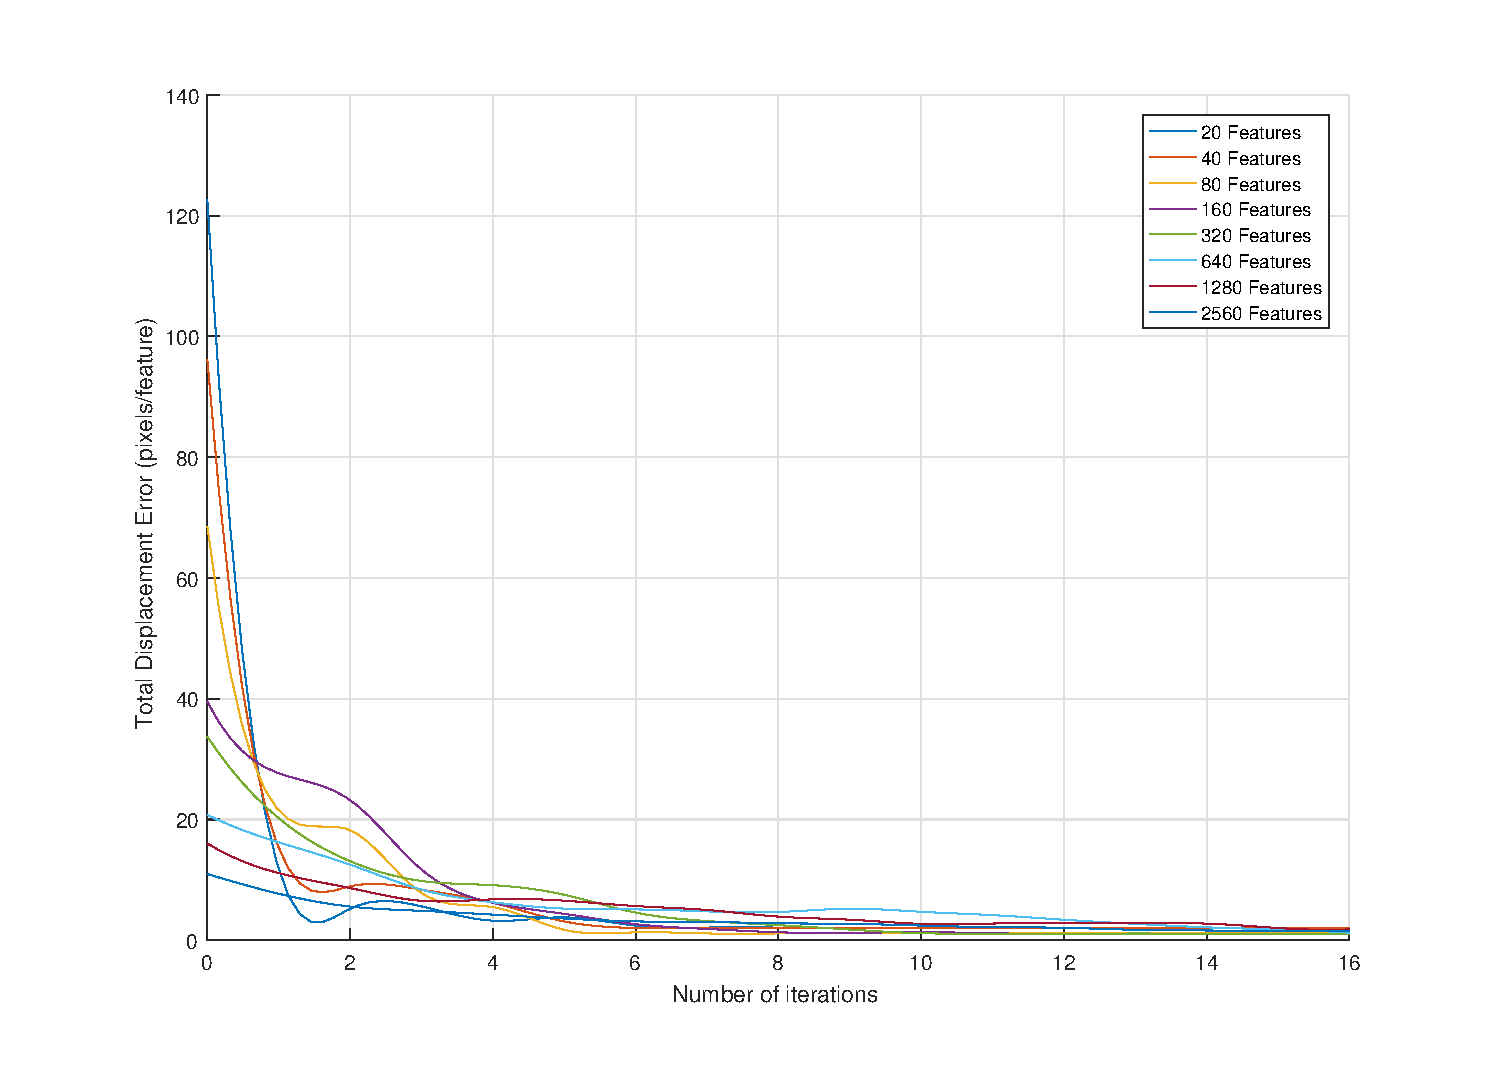
\includegraphics[width=\textwidth]{figures/alignment/error_for_iterations}
	\caption{The error in pixels per feature for performing $n$ iterations of the iterative closest point algorithm on differently sized sets of the strongest feature points}
	\label{fig_results_error_plot}
\end{figure}

Figure \ref{fig_alignment_results} shows the alignment between the transform and reference image when certain numbers of feature points are selected and used to compute the transform. It can be observed that $20$ features is not sufficient to compute a mapping, but that all of the images with more than $40$ features are imperfectly aligned. This is in spite of the fact that iterative closest point converges to a local minimum in terms of displacement error.

From this, it can be concluded that selecting a small, but sufficient number of feature points produces optimal alignment. This is likely due to the fact that additional feature points beyond just the strongest features in the images introduce error by trying to align the noisier parts of the background. A better error metric may be the one shown in Figure \ref{fig_results_alignment_error_plot} which shows the error in terms of the intensity difference. The magnitude of the overlaid image subtracted from the original is used to compute this error metric which more accurately reflects the alignment results shown in Figure \ref{fig_alignment_results}.

\begin{figure}[h]
	\centering
	\begin{subfigure}[b]{0.3\textwidth}
		\centering
		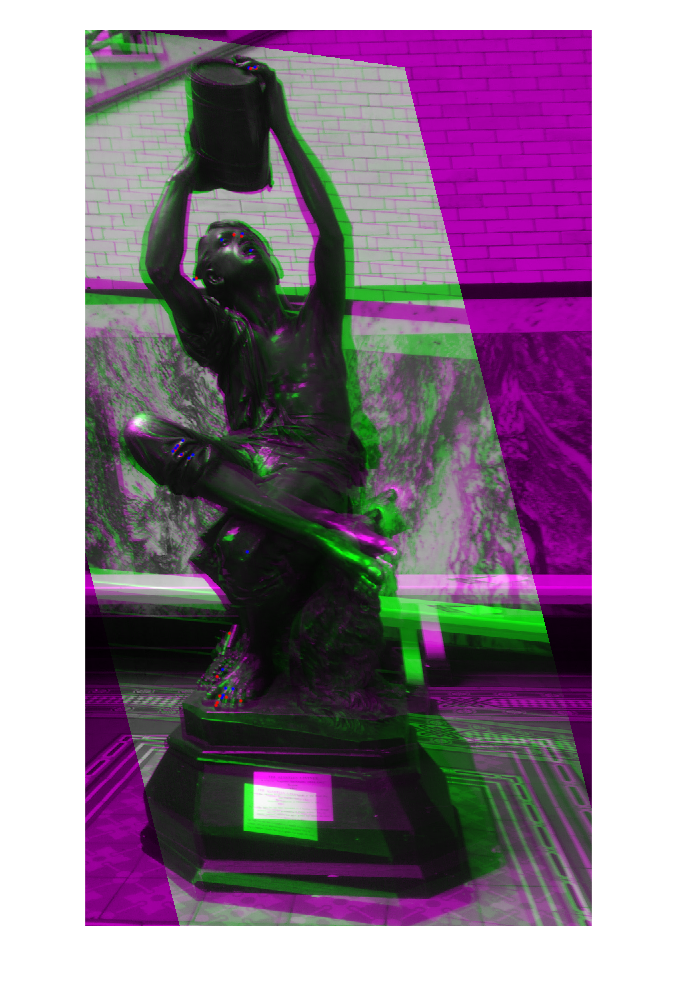
\includegraphics[width=\textwidth]{figures/alignment/fused_20_features_16_iterations}
		\caption{20 features}
	\end{subfigure}
	\begin{subfigure}[b]{0.3\textwidth}
		\centering
		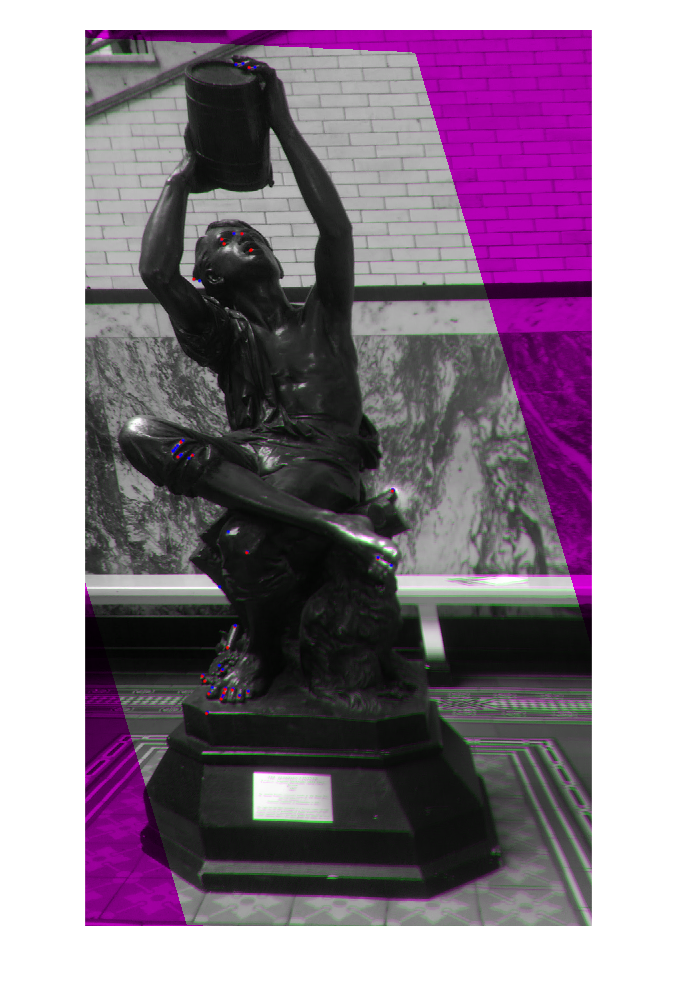
\includegraphics[width=\textwidth]{figures/alignment/fused_40_features_16_iterations}
		\caption{40 features}
	\end{subfigure}
	\begin{subfigure}[b]{0.3\textwidth}
		\centering
		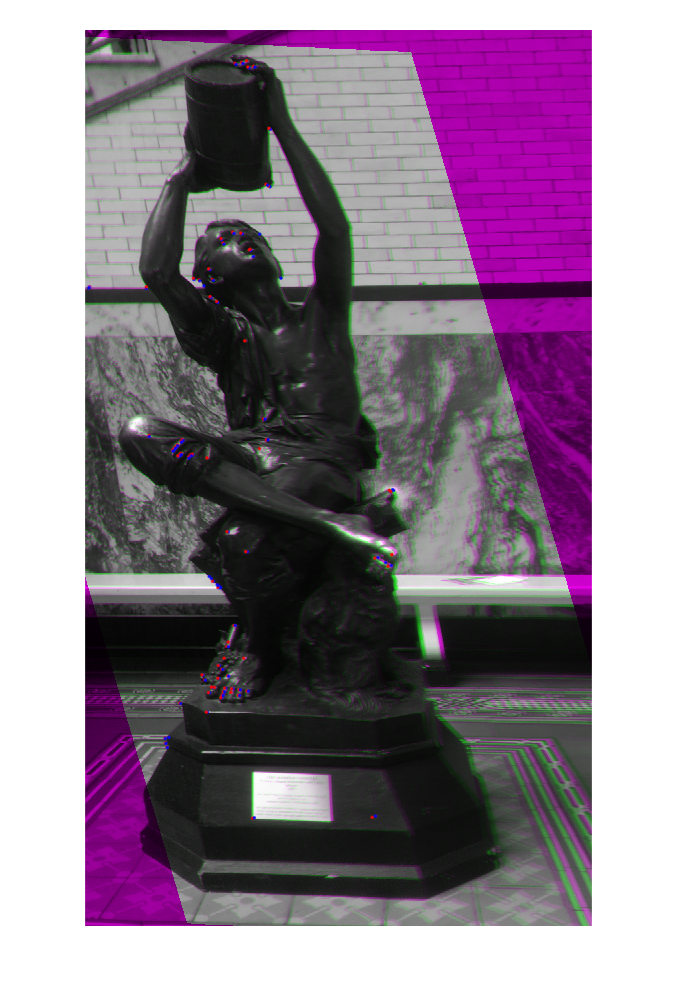
\includegraphics[width=\textwidth]{figures/alignment/fused_80_features_16_iterations}
		\caption{80 features}
	\end{subfigure}

   	\begin{subfigure}[b]{0.3\textwidth}
    	\centering
    	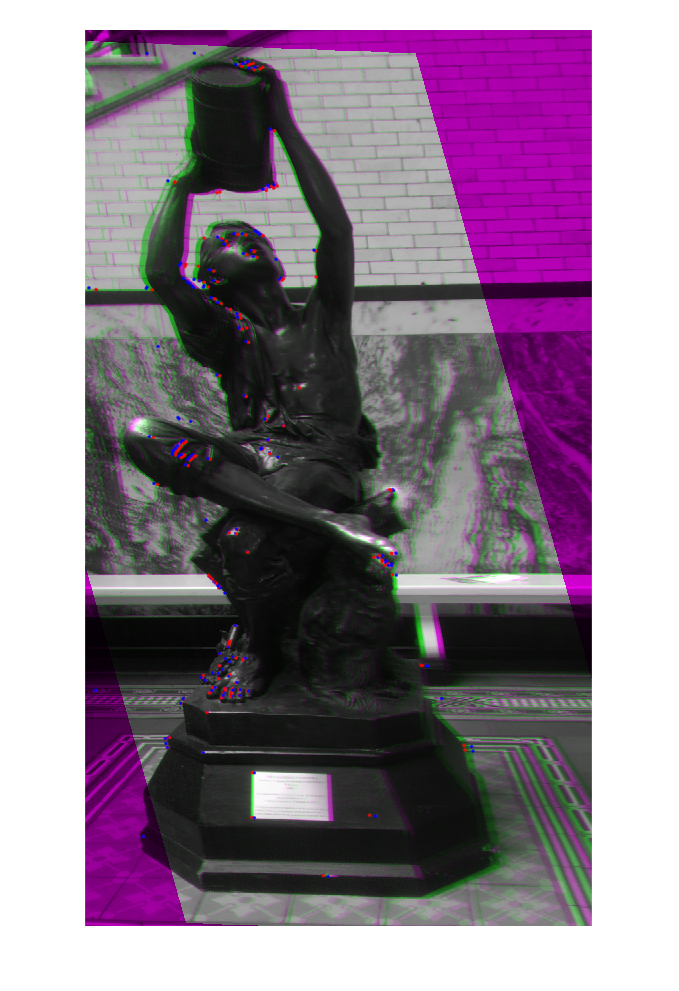
\includegraphics[width=\textwidth]{figures/alignment/fused_160_features_16_iterations}
    	\caption{160 features}
    \end{subfigure}
    \begin{subfigure}[b]{0.3\textwidth}
    	\centering
    	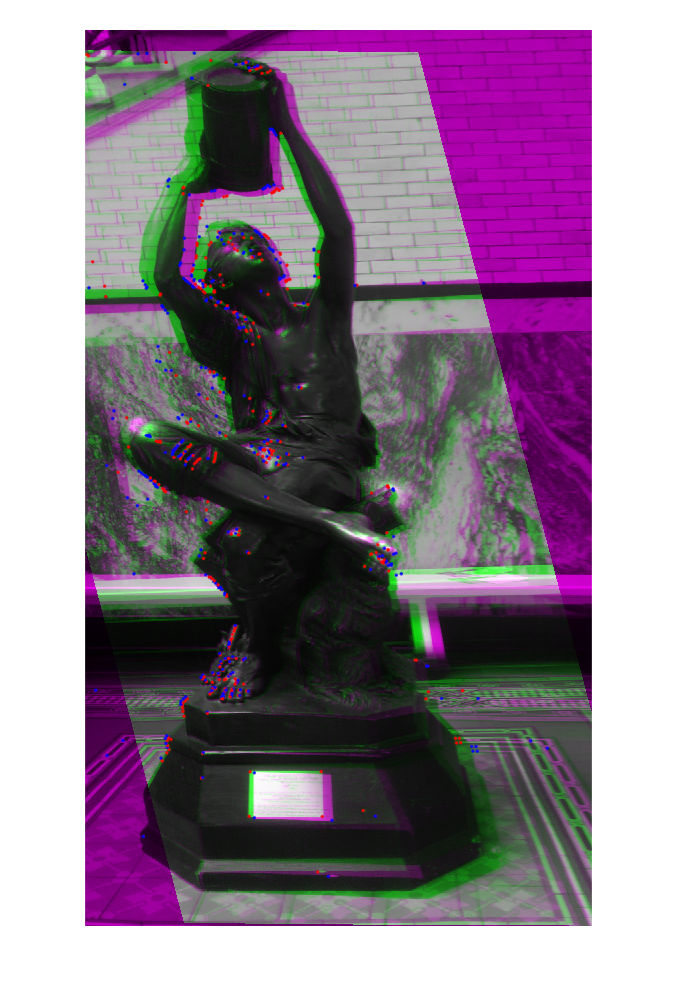
\includegraphics[width=\textwidth]{figures/alignment/fused_320_features_16_iterations}
    	\caption{320 features}
    \end{subfigure}
    \begin{subfigure}[b]{0.3\textwidth}
    	\centering
    	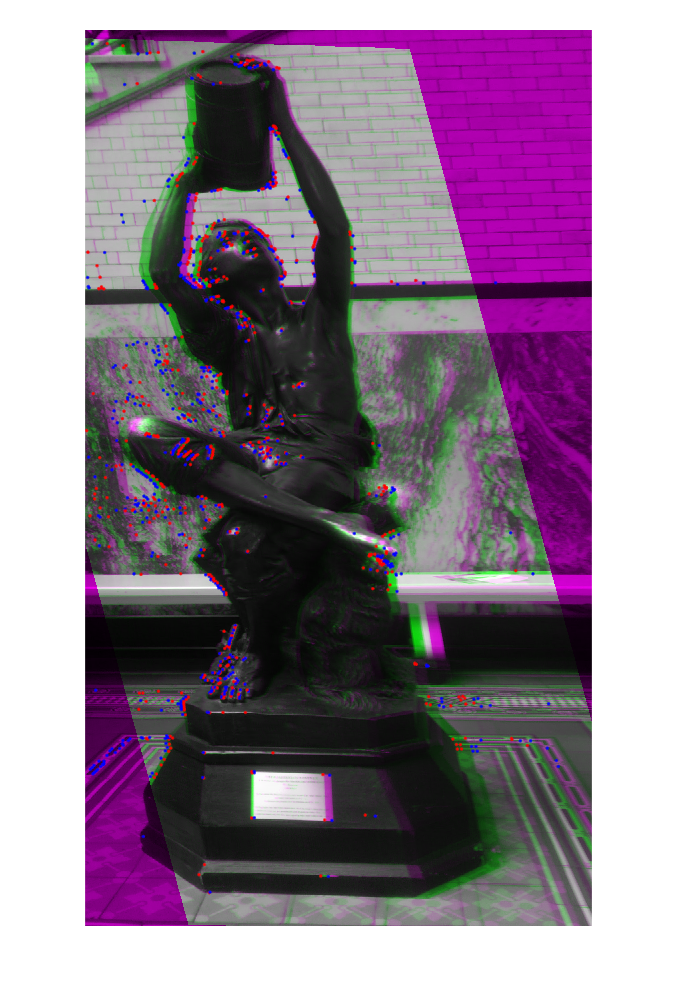
\includegraphics[width=\textwidth]{figures/alignment/fused_640_features_16_iterations}
    	\caption{640 features}
    \end{subfigure}
	\caption{Alignment results after running iterative closest point for 16 iterations on varying numbers of features with reference features marked in red and transformed features in blue}
	\label{fig_alignment_results}
\end{figure}

\begin{figure}[h]
	\centering
	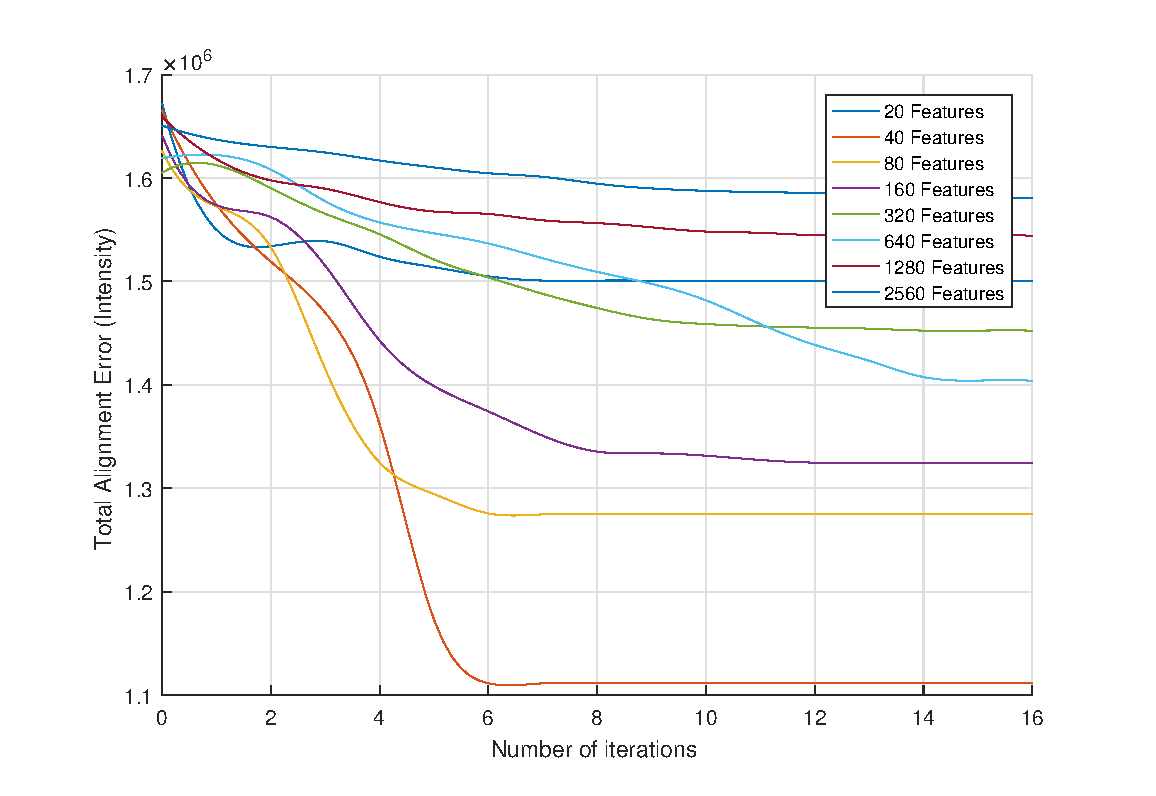
\includegraphics[width=\textwidth]{figures/alignment/error_for_alignment}
	\caption{The error in intensity based on the alignment from performing $n$ iterations of the iterative closest point algorithm on differently sized sets of the strongest feature points}
	\label{fig_results_alignment_error_plot}
\end{figure}

\subsection{Implemented Design Details}

The implemented design for detecting feature points and transform the data for alignment and fusion can be seen in Figure \ref{fig_implemented}. The timing, power, and utilization data can be found in Tables \ref{table_timing}, \ref{table_power}, and \ref{table_utilization} respectively.

\begin{figure}[h]
	\centering
	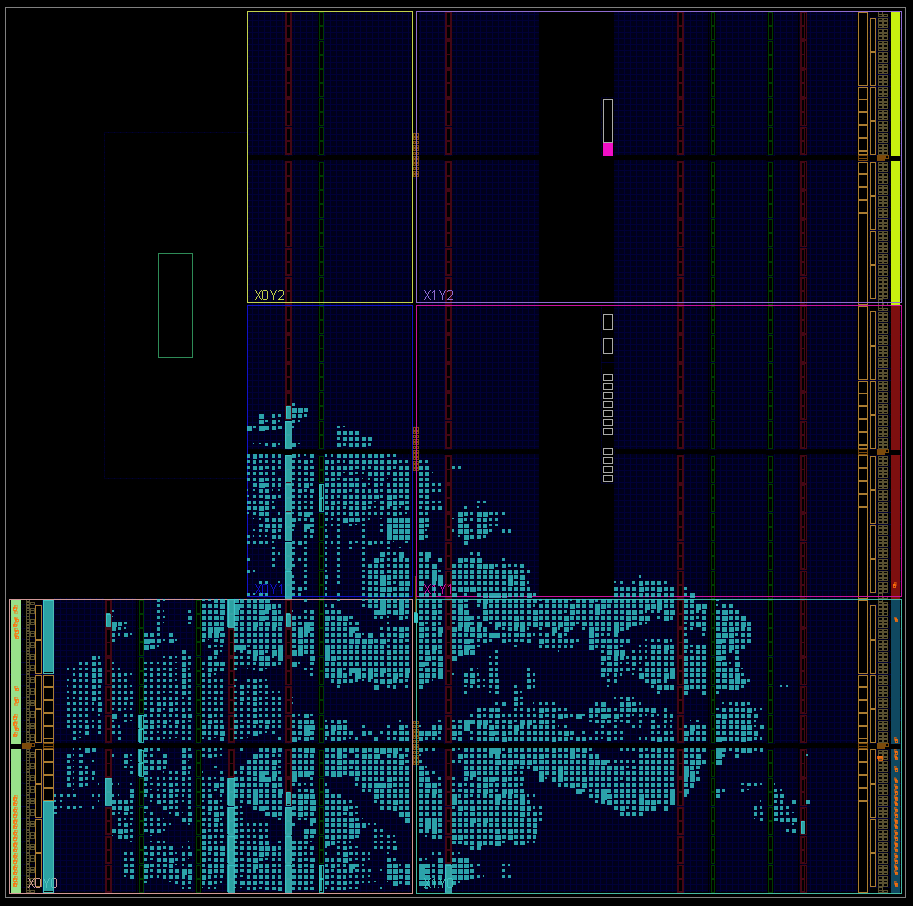
\includegraphics[width=0.8\textwidth]{figures/pictures/implemented}
	\caption{FPGA implemented design for live fusion using feature point detection}
	\label{fig_implemented}
\end{figure}

\begin{table}[h]
	\centering
	\caption{Timing data for the implemented design}
	\begin{tabular}{l|l}
		Worst Case Slack (Setup) & $+0.081 ns$ \\
		\hline
		Worst Case Slack (Hold) & $+0.047 ns$ \\
		\hline
		Total \# of Endpoints & $4495$
	\end{tabular}
	\label{table_timing}
\end{table}

\begin{table}[h]
	\centering
	\caption{Power data for the implemented design}
	\begin{tabular}{l|l}
		Total On-Chip Power & $0.615 W$ \\
		\hline
		Junction Temperature & $32.1 ^{\circ} C$ 
	\end{tabular}
	\label{table_power}
\end{table}

\begin{table}[h]
	\centering
	\caption{Utilization data for the implemented design}
	\begin{tabular}{l|l}
		Look-up Table & $8758$ \\
		\hline
		Flip-flops & $6645$ \\
		\hline
		Block-RAM & $22$
	\end{tabular}
	\label{table_utilization}
\end{table}

\section{Conclusions}

The approach presented is capable of performing the task stated in the abstract in real time. Careful pipelining in a novel architecture for the computing of the hessian determinants makes this possible. The treatment of each frame as a generation of feature points to be transformed to a local error minimum as opposed to a more rigid architecture of performing multiple iterations on one feature set helps alleviate the overhead of the design, and make it realizable. The available chipset was not of sufficient size to perform the larger corrections of scale and shear due to the prohibitive nature of instantiating large arrays of SVD solving cells. However, on a more robust chipset, scale and shear should also be correctable factors, as well as giving the ability to compute the transform from a larger set of feature points.

\pagebreak
\clearpage

\singlespacing

\bibliographystyle{plain}
\bibliography{thesis}

\end{document}
